%------------------------------------------------------------------------------
%	TOY PROBLEM
%------------------------------------------------------------------------------

\subsection{Toy Problem}

%------------------------------------------------------------------------------
%	PROBLEM DESCRIPTION
%------------------------------------------------------------------------------

\subsubsection{Problem Description} \label{toyDescSec}

Now that the general framework of this project has been explained, a simple case, i.e. a "toy" problem, is chosen in order to further elaborate on the proposed algorithm in a more streamlined manner, but also to make a first assessment of its efficiency, drawbacks, and future issues that need to be adjusted. Therefore, a \gls{SDOF} oscilator is selected, with its stiffness being the deterioration parameter. The mass of the oscilator, $m$, is assumed to be deterministic and constant, while the initial stiffness is denoted as $K_0$. The described system is illustrated in Figure \ref{sdofOscil}.

\begin{figure}[H]
    \centering
	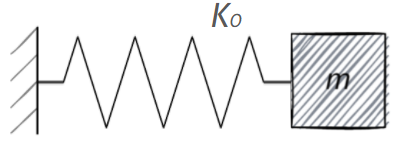
\includegraphics[width=0.3\linewidth]{Figures/SDOFoscilator.png}
	\caption{\gls{SDOF} oscillator}
	\label{sdofOscil}
\end{figure}

The deterioration model employed is:

\begin{equation}
    D(\tau) = A \, \tau^B
\end{equation}

where $A$, $B$, are random variables, responsible for the uncertainty in this model. In particular, $A$ corresponds to the deterioration rate, while $B$ is related to the non-linearity effect in terms of a power law in time. This is a standard model, described by the rate equation above, often employed for an engineering system's deterioration, e.g. \cite{kamariotis2022value}.\\

A clear distinction should be made between the decision step $t$, which is the running time variable of the system's lifespan, and the deterioration rate $\tau$ which describes the exposure time, or the age, of the system, and subsequently the degree to which the corrosive environment affects it. In a scenario where no maintenance action is performed during the time window of interest, $t$ and $\tau$ coincide. However, as will be displayed in this section, the agent's actions can possibly reduce or even reset the deterioration rate $\tau$ while the decision step $t$ will keep increasing with unit step.\\

The stiffness at any given state is calculated as follows:

\begin{equation}
    K(\tau) = \cfrac{K_0}{1+D(\tau)} = \cfrac{K_0}{1+A\,\tau^B}
\end{equation}

It is assumed that there is a monitoring system, whose noisy measurements are passed through an \gls{OMA} scheme, which subsequently outputs modal data, in this case, the eigenfrequency, $\omega$. The eigenfrequency, as known from basic structural dynamics theory, is calculated, hence related to the system's damage, through Equation \ref{omegaEq}. 

\begin{equation}
    \hat{\omega} (\tau) = \sqrt{\cfrac{K(\tau)}{m}} = \sqrt{\cfrac{K_0}{m \, \left ( 1 + D(\tau) \right )}} = \sqrt{\cfrac{K_0}{m \, \left ( 1 + A \, \tau^B \right )}} \label{omegaEq}
\end{equation}

Since $A$ and $B$ are stochastic, $\hat{\omega}(\tau)$ represents the aforementioned noisy measurement. After passing it through the the \gls{OMA} procedure, the yielded observation which is given to the agent can be expressed as:

\begin{equation}
    \omega (\tau ) = \hat{\omega}(\tau ) + \varepsilon_{\text{oma}} \label{noisyObs}
\end{equation}

where $\varepsilon _{\text{oma}}$ corresponds to the additional noise that is explicitly added during the \gls{OMA} scheme.\\

For the case at hand, it is assumed that the additional noise $\varepsilon _{\text{oma}}$ follows a Gaussian distribution with a zero mean and a standard deviation that is proportional to the noisy measurement. 

\begin{equation}
    \varepsilon _{\text{oma}} \sim \ccal{N} \left( 0, \,\, \epsilon _{\text{c}} \cdot \hat{\omega}(\tau) \right)
\end{equation}

where $\epsilon_{\text{c}}$ is a coefficient describing the degree to which the \gls{OMA} scheme contaminates the measurement with noise.\\

Therefore, the observation during each decision step is generated based on the following Gaussian distribution:

\begin{equation}
    \omega (\tau) \sim \ccal{N}\left ( \hat{\omega}(\tau) , \,\, \epsilon_{\text{c}} \cdot \hat{\omega}(\tau) \right) \label{obsDistr}
\end{equation}

The choice for the possible actions that the agent can take is a significant modeling decision. Apart from the "\textit{do nothing}" and the "\textit{total replacement}" actions, there is the need of a "\textit{partial repair}" one, too. The way in which the rest of the parameters will be affected due to such a repair can vary depending on the materials of the structure, the type of repair, etc. Regarding the chosen deterioration model, i.e. $D(\tau) = A\, \tau^B$, there are three cases of partial repair that can be distinguished.

\begin{itemize}
    \item Reduce only the caused damage $D(\tau)$, but the deterioration rate, $\tau$, at which the environment affects the structure, stays the same. This would mean that the slope of the $D(\tau)-\tau$ curve will stay the same, and a vertical shift of the right-half curve will be observed, as displayed in Figure \ref{repair1}. This could be the case when restoring the damaged surrounding concrete of a \gls{RC} component, but no action is taken for the corrosion of the rebar, which will continue to develop.
    \item Reduce the deterioration rate, meaning that the environment will continue to affect the structure with a reduced intensity, but the existent damage that is already caused is not affected. Geometrically, there will be a horizontal shift to the left in order for the damage to continue developing in a less steep slope (Figure \ref{repair2}). For example, applying an epoxy painting on a steel member without repairing the existent damage, will slow down the effect of the corroding environment, but the damaged cross-section will remain as is.  
    \item A combination of the two cases above, which means that both the damage $D(\tau)$ and the deterioration rate, $\tau$, are reduced. This action equals a move back along the $D(\tau) - \tau$ curve as illustrated in Figure \ref{repair3}. For example, removing/restoring the corroded parts of a steel cross-section and applying a protective paint to protect it against the corroding environment.
\end{itemize}

\begin{figure}[H]
    \centering
    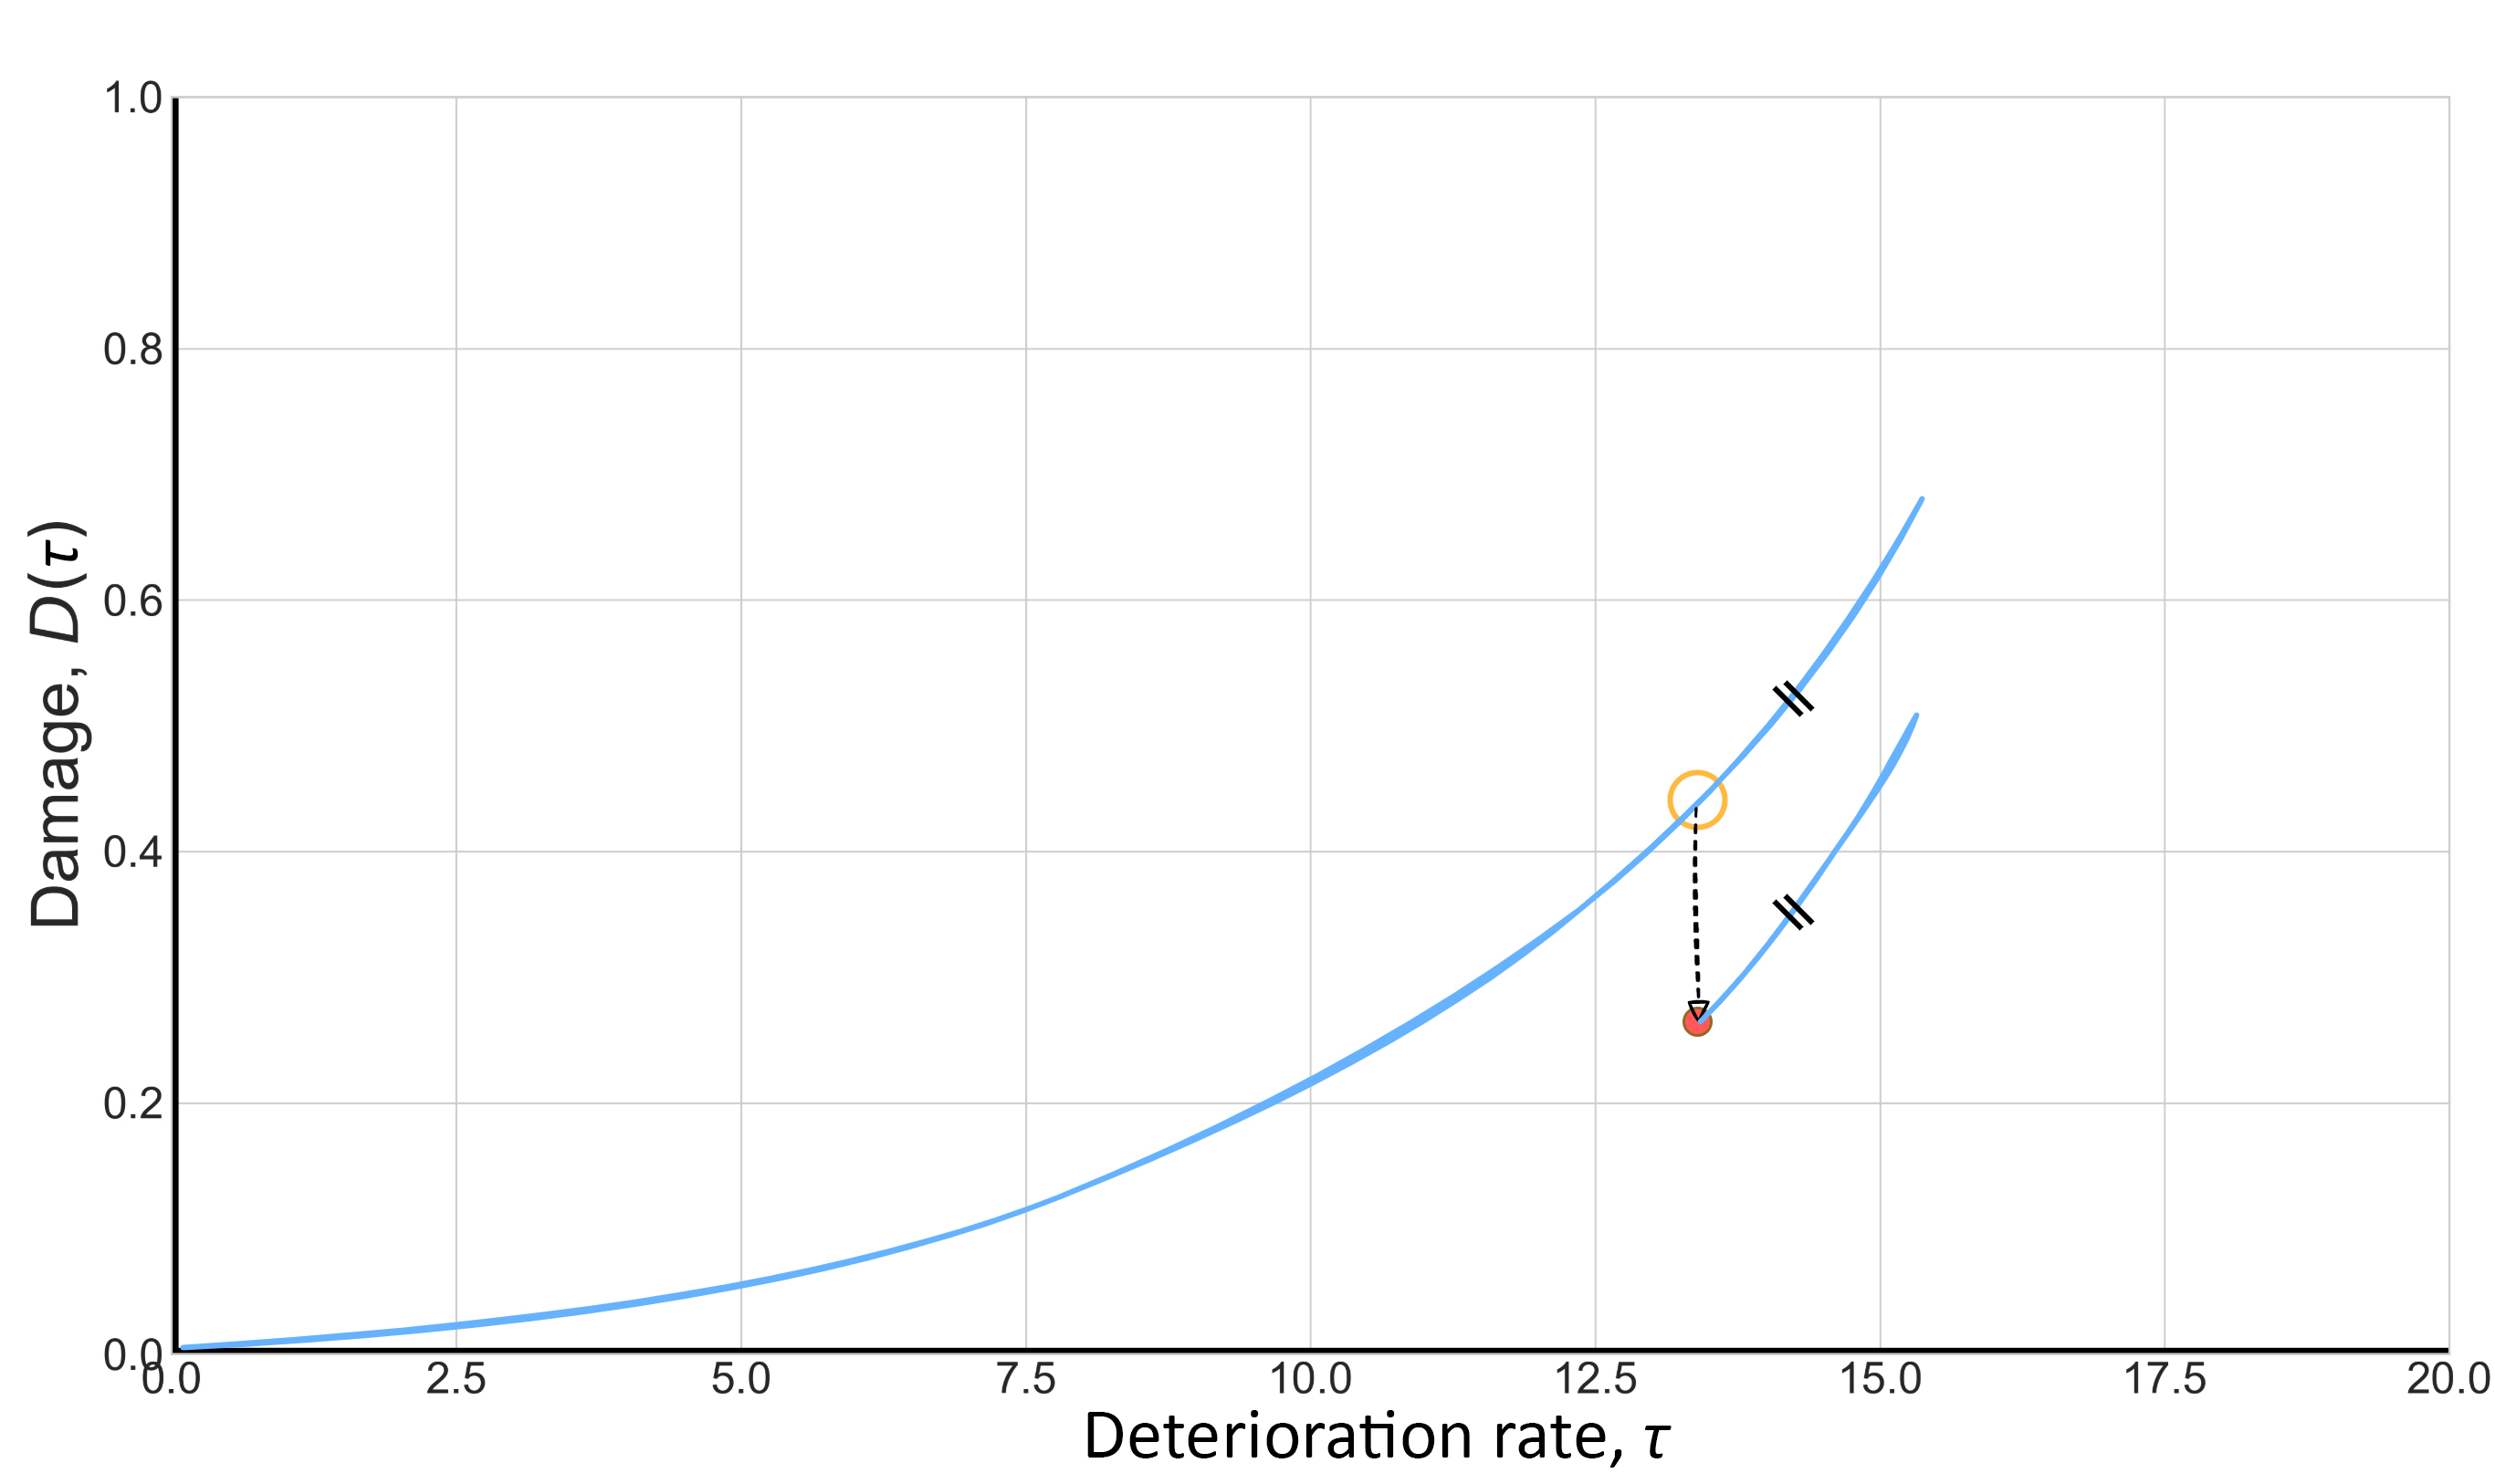
\includegraphics[width=0.8\textwidth]{Figures/repair1.jpg}
    \caption{Repair by reducing the damage $D(\tau)$}
    \label{repair1}
\end{figure}

\begin{figure}[H]
    \centering
    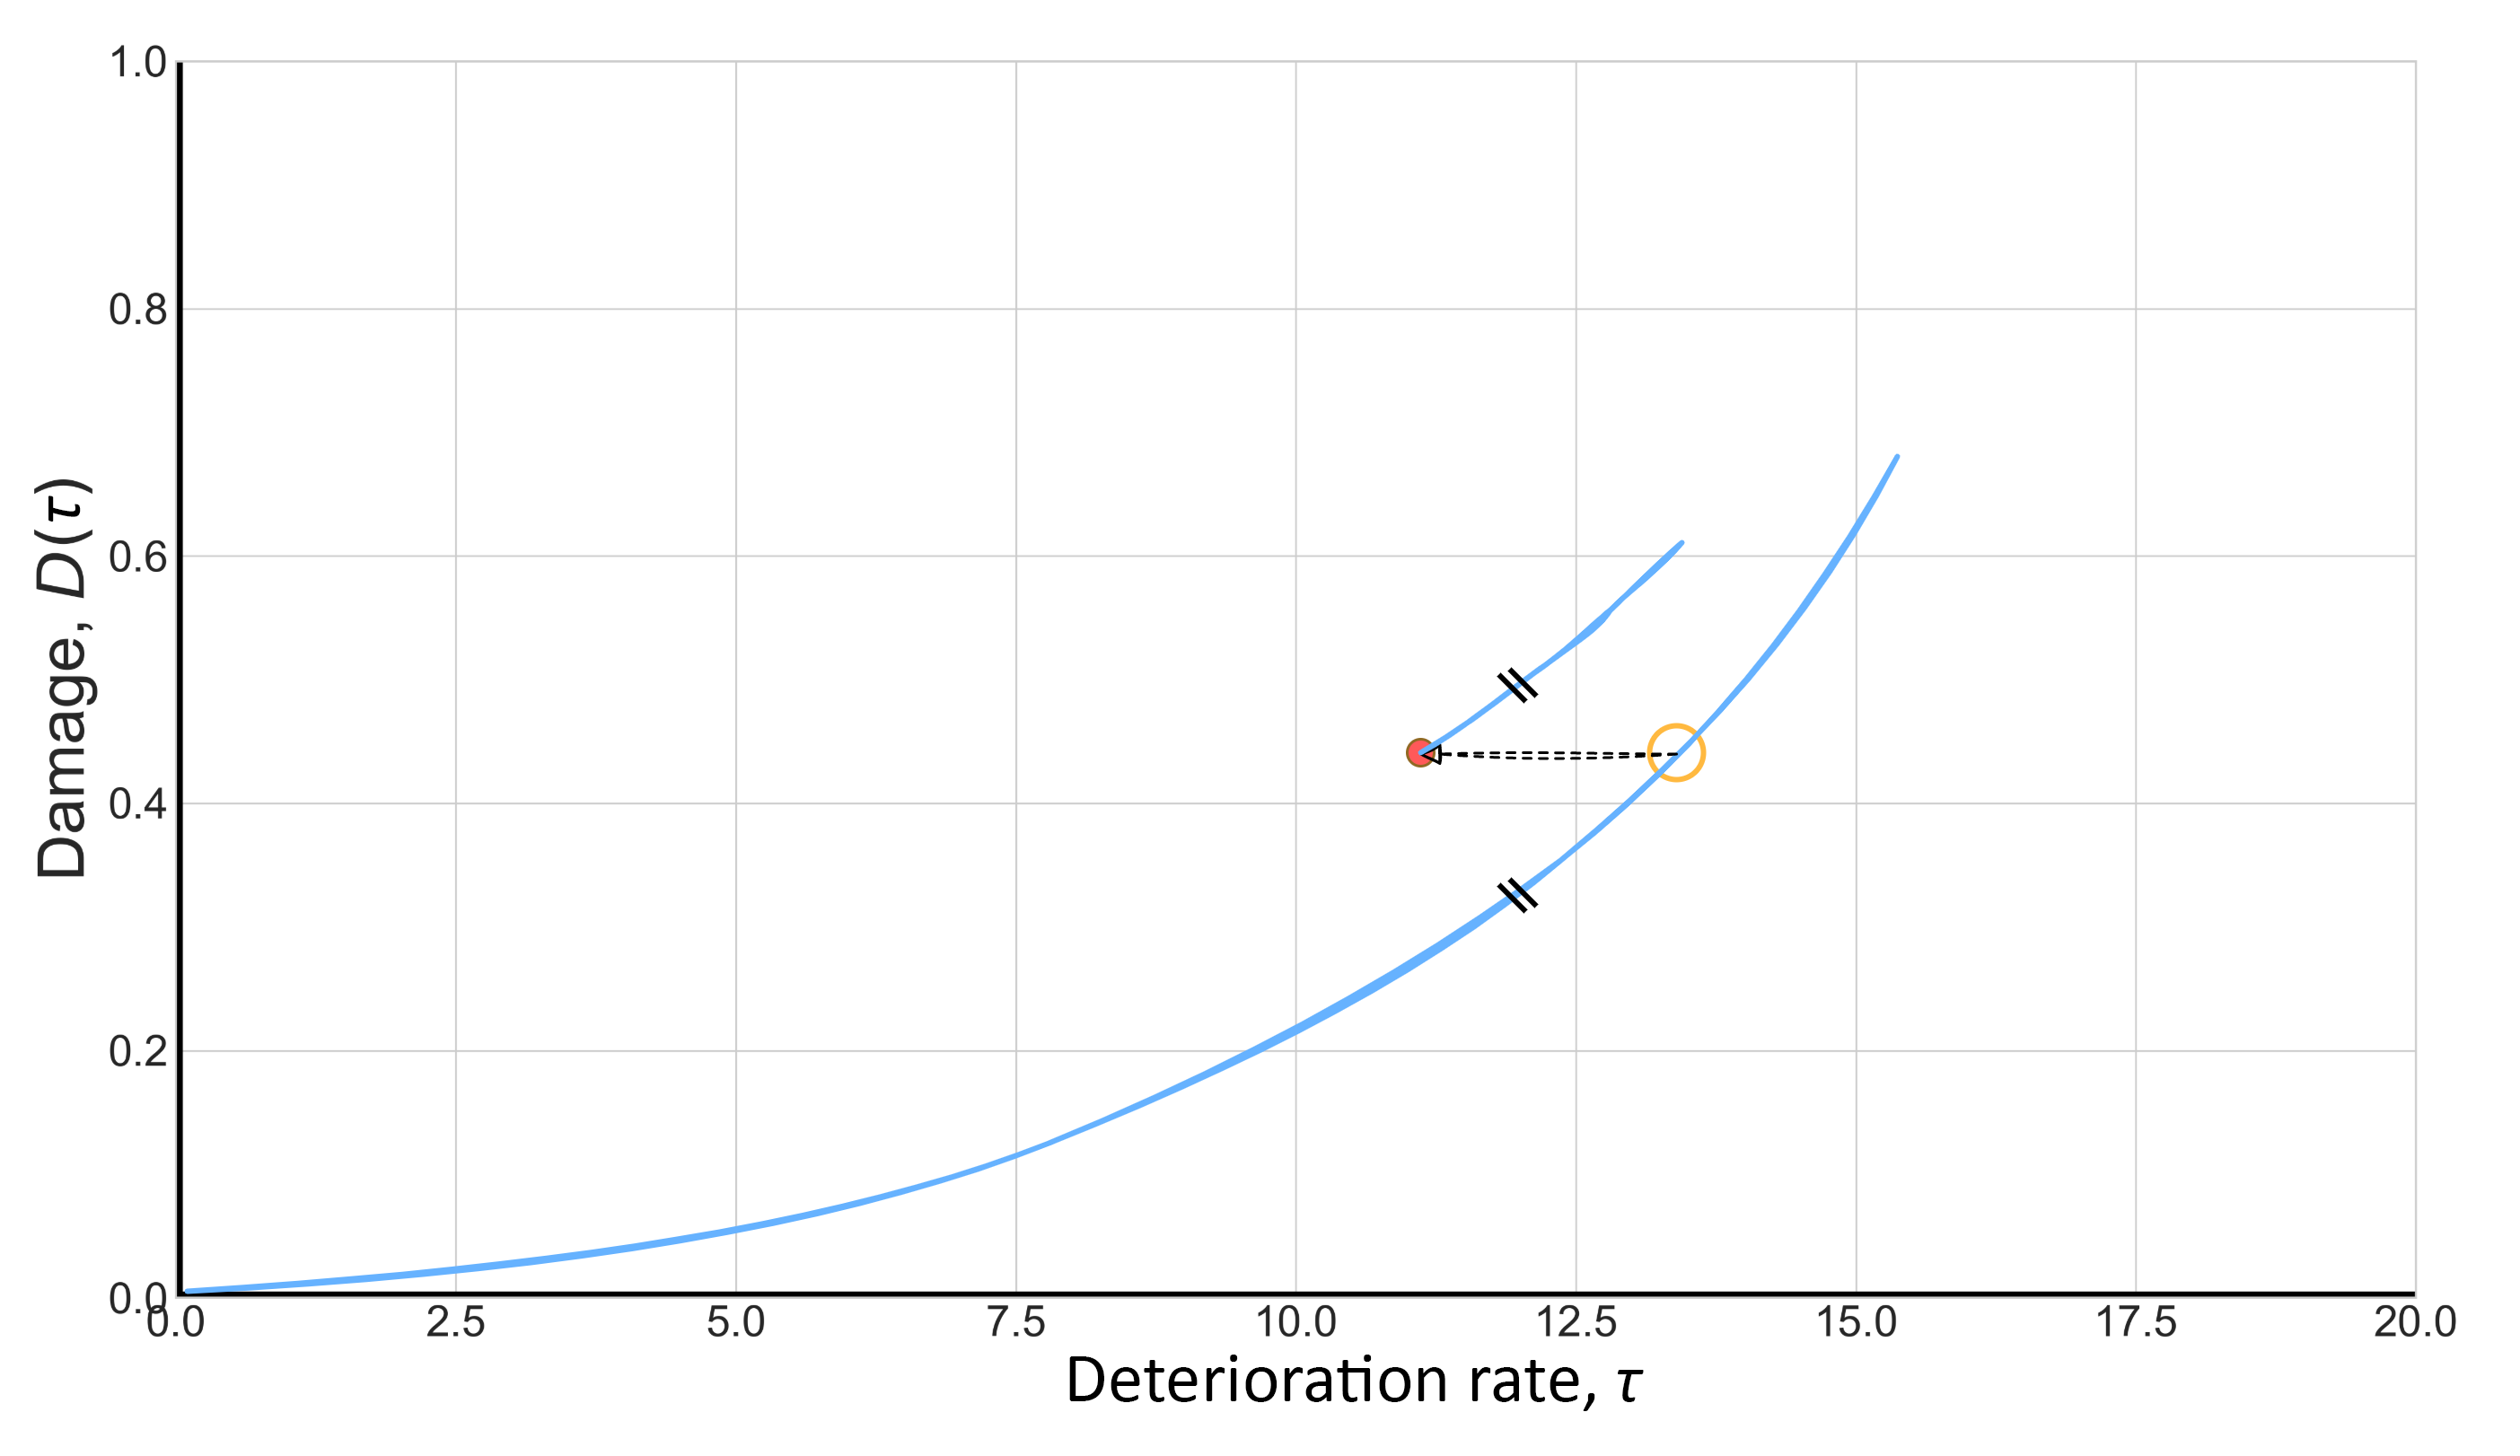
\includegraphics[width=0.8\textwidth]{Figures/repair2.png}
    \caption{Repair by reducing the deterioration rate $\tau$}
    \label{repair2}
\end{figure}

\begin{figure}[H]
    \centering
    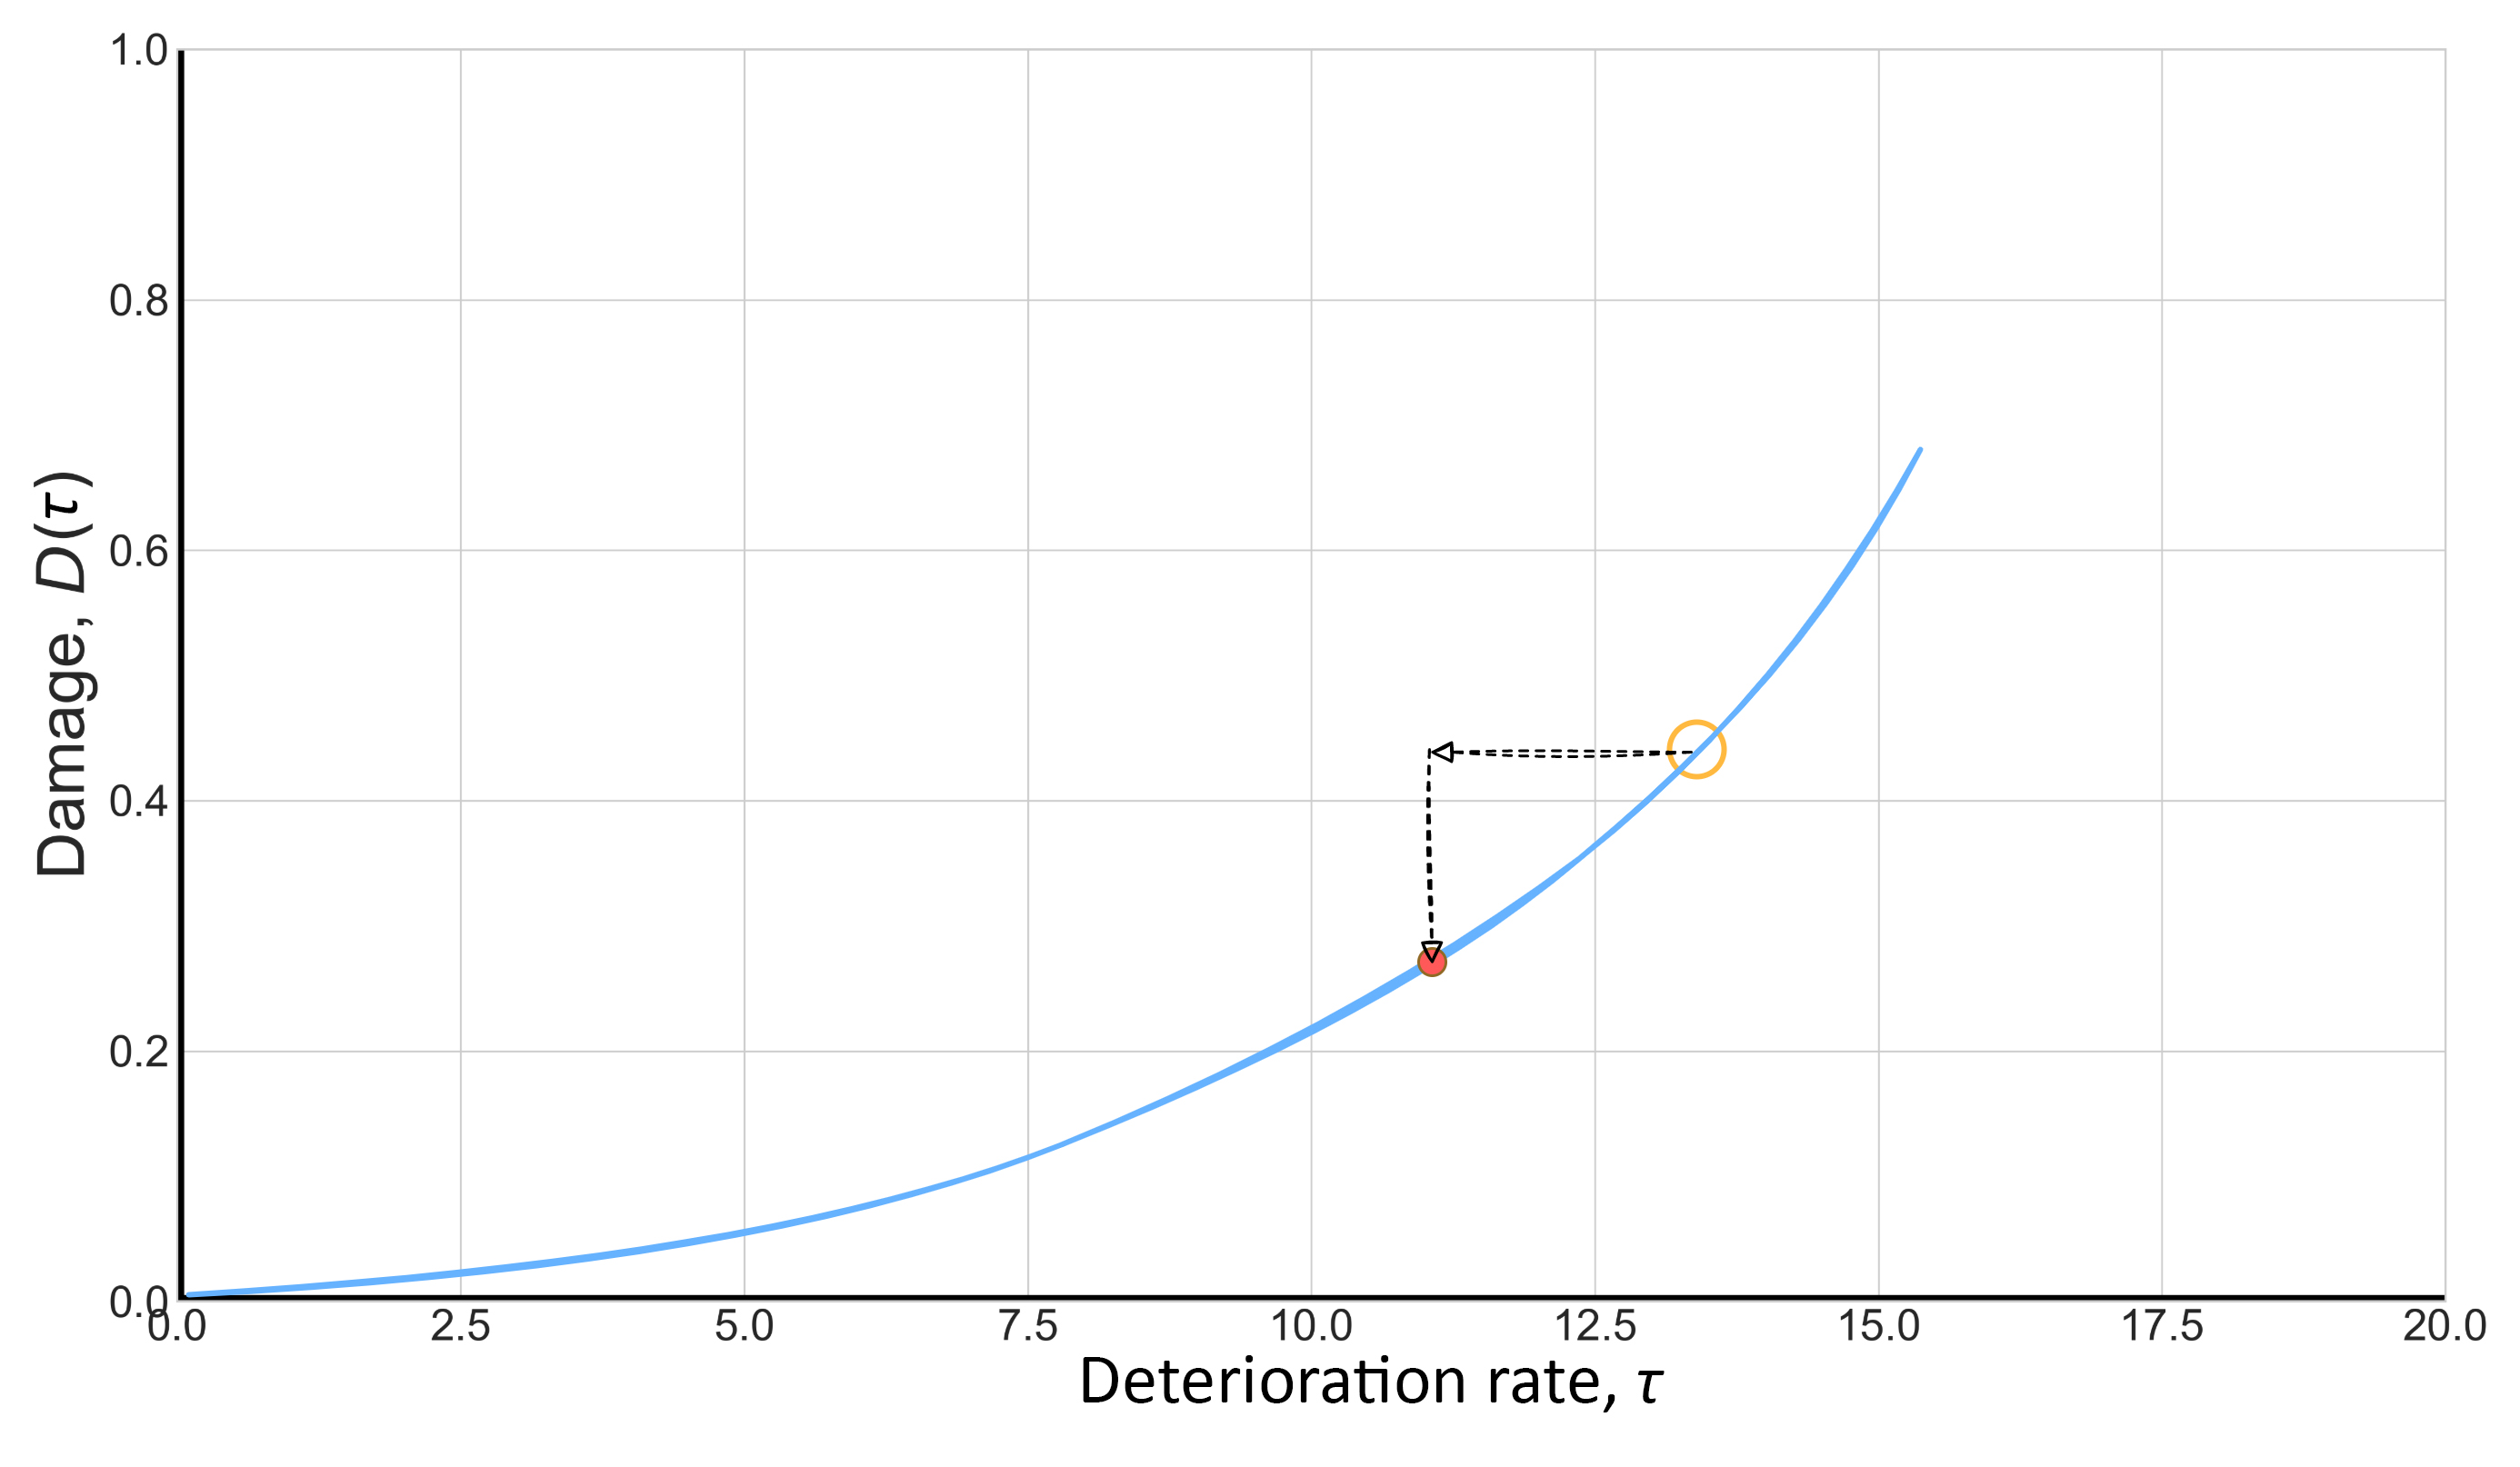
\includegraphics[width=0.8\textwidth]{Figures/repair3.jpg}
    \caption{Repair by reducing both the damage and the deterioration rate}
    \label{repair3}
\end{figure}

Having described the various approaches for modelling a repair action, the one depicted in Figure \ref{repair2} is chosen for the current application. Thus, the three possible actions are listed in Table \ref{actToy}.

\begin{table}[H]
    \centering
    \caption{Action-space for toy problem}
    \label{actToy}
    \begin{threeparttable}
        \begin{tabular}{cc}
            \toprule
            \textbf{Index} & \textbf{Action} \\ \midrule
            0 & do nothing \\
            1 & partial repair\tnote{*} \\
            2 & total replace \\ \bottomrule
        \end{tabular}
        \begin{tablenotes}
            \item[*] \footnotesize{Decrease the deterioration rate $\tau$, i.e. rewind by two steps}
        \end{tablenotes}
    \end{threeparttable}
\end{table}


Regarding the rewards, i.e. the costs of maintenance, a fixed amount is considered for the system's total replace (action 2), and every other cost is expressed as relatively to this value. The correlation between the costs is included in Table \ref{costToy}.

\begin{table}[H]
    \centering
    \caption{Rewards (costs) for the toy problem}
    \label{costToy}
    \begin{tabular}{lccc}
        \toprule
        \textbf{Description} & \textbf{Cost} & \textbf{Value} & \textbf{Factor} \\ \midrule
        Total replacement & $C_{\text{R}}$ & $C_0$ units & $1$ \\ 
        Partial repair & $C_{\text{M}}$ & $0.5\, C_{\text{R}}$ & $0.5$ \\
        Failure & $C_{\text{F}}$ & $2\, C_{\text{R}}$ & $2$ \\ 
        Risk of failure & $C_{\text{risk}}$ & $P_f\,C_{\tet{F}}$ & $2\,P_f$ \\ \bottomrule
    \end{tabular}
\end{table}

It can be observed that failure, which will cause a complete replacement of the component (system), has a higher cost than the actual replacement as an action. This is the case because of the sudden aspect of a structure failing, and the unpredicted consequences that this event might provoke financially.\\

The input data used for this application, such as deterministic quantities, starting values, etc, are gathered and displayed in Table \ref{toyInput}.

\begin{table}[H]
    \centering
    \caption{Toy problem input data}
    \label{toyInput}
    \begin{tabular}{lcc}
        \toprule
        \textbf{Quantity}             & \textbf{Value}    & \textbf{Units} \\ \midrule
        Mass, $m$                     & $10$              & {[}kg{]}       \\
        Initial stiffness, $K_0$      & $200$             & {[}N/m{]}      \\
        Replace cost, $C_R$           & $10000$           & {[}-{]}        \\
        Noise coefficient, $\epsilon _{\text{c}}$ & $10\%$ \tnote{*}  & {[}-{]}        \\ \bottomrule
    \end{tabular}
\end{table}


%------------------------------------------------------------------------------
%	DISCRETE CASE
%------------------------------------------------------------------------------

\subsubsection{Discrete case}

Considering the stochastic parameters $A, B$, as well as the damage $D(\tau)$ to be continuous variables, increases significantly the computational cost. This is why, in order to scale up gradually the complexity in verifying the validity of the proposed methodology, a discrete version of the described toy problem is being tackled first.\\

In particular, the following discrete values are accounted for:

\begin{gather*}
    A = 
    \begin{bmatrix}
        6 \scnot{-4} & 8 \scnot{-4} & 10 \scnot{-4} & 12 \scnot{-4} & 14 \scnot{-4}
    \end{bmatrix} \\
    B = 
    \begin{bmatrix}
        1.4 & 1.6 & 1.8 & 2.0 & 2.2
    \end{bmatrix} \\
    D = 
    \begin{bmatrix}
        0 & 0.1 & 0.2 & 0.3 & 0.4 & 0.5 & 0.6 & 0.7 & 0.8 & 0.9 & 1.0
    \end{bmatrix}
\end{gather*}

It should be noted that just for demonstration purposes in the coming figures, smaller discrete spaces will be used, particularly:

\begin{gather*}
    A = 
    \begin{bmatrix}
        A_1 & A_2
    \end{bmatrix} \\
    B = 
    \begin{bmatrix}
        B_1 & B_2
    \end{bmatrix} \\
    D = 
    \begin{bmatrix}
        D_1 & D_2 & D_3
    \end{bmatrix}
\end{gather*}


In each iteration the agent does not know the exact value of the damage, so it forms a belief $\underline{b}$, i.e. a vector which contains the probabilities of all possible damage states\footnote{The sum of all elements in the belief vector should sum up to 1, i.e. $\sum b_i = 1$.}. For the smaller scale representative discrete case, this vector has the form displayed in Figure \ref{beliefDisc}. 

\begin{figure}[H]
    \centering
	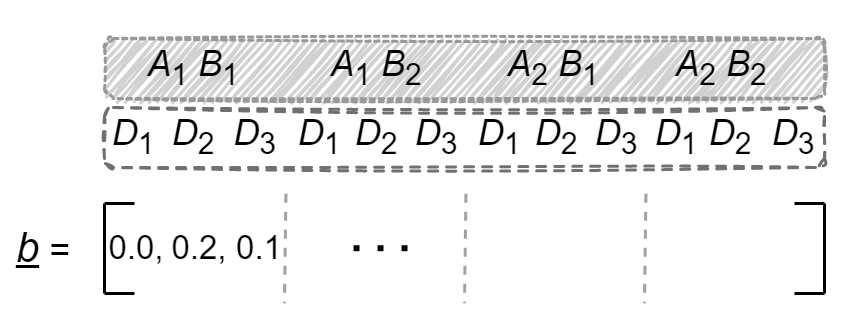
\includegraphics[width=0.5\linewidth]{Figures/beliefDiscrete.png}
	\caption{Belief vector, $\underline{b}$ for discrete case}
	\label{beliefDisc}
\end{figure}

The observation $\omega (\tau)$ in each decision step is generated as described already in Equation \ref{obsDistr}.\\

The main advantage of this simplification, compared to the continuous case, is the calculation of the belief vector in a closed-form. This is achieved using the so-called transition matrix $\underline{\underline{\mathbb{P}}}$, as well as the observation matrix $\underline{\underline{\mathbb{O}}}$. The former corresponds to the probability of shifting to a new state given the previous state and the chosen action, while the latter reflects the probability of an eigenfrequency $\omega$ to be observed given the current state. In math notation, they are defined as follows:

\begin{gather}
    \underline{\underline{\mathbb{P}}} = \prob{s_{t+1} \mid s_t, a_t} \\
    \underline{\underline{\mathbb{O}}} = \prob{o_t \mid s_t}
\end{gather}

where $s_{t+1}$ is the next state, $s_t$ is the current state, $a_t$ is the chosen action and $o_t$ is the observation $\omega$.\\

The dependency of the transition probability to the chosen action is dropped, since $a_t$ is accounted for by modifying the deterioration rate. Additionally, in order to describe all possible transitions, a different transition matrix is considered for each deterioration rate $\tau$, i.e. $\underline{\underline{\mathbb{P}_{\tau}}} = \prob{s_{t+1} \mid s_t}$.

\newpage

A typical example of a transition matrix for a random deterioration rate is depicted in Figure \ref{transMatDisc}.

\begin{figure}[H]
    \centering
	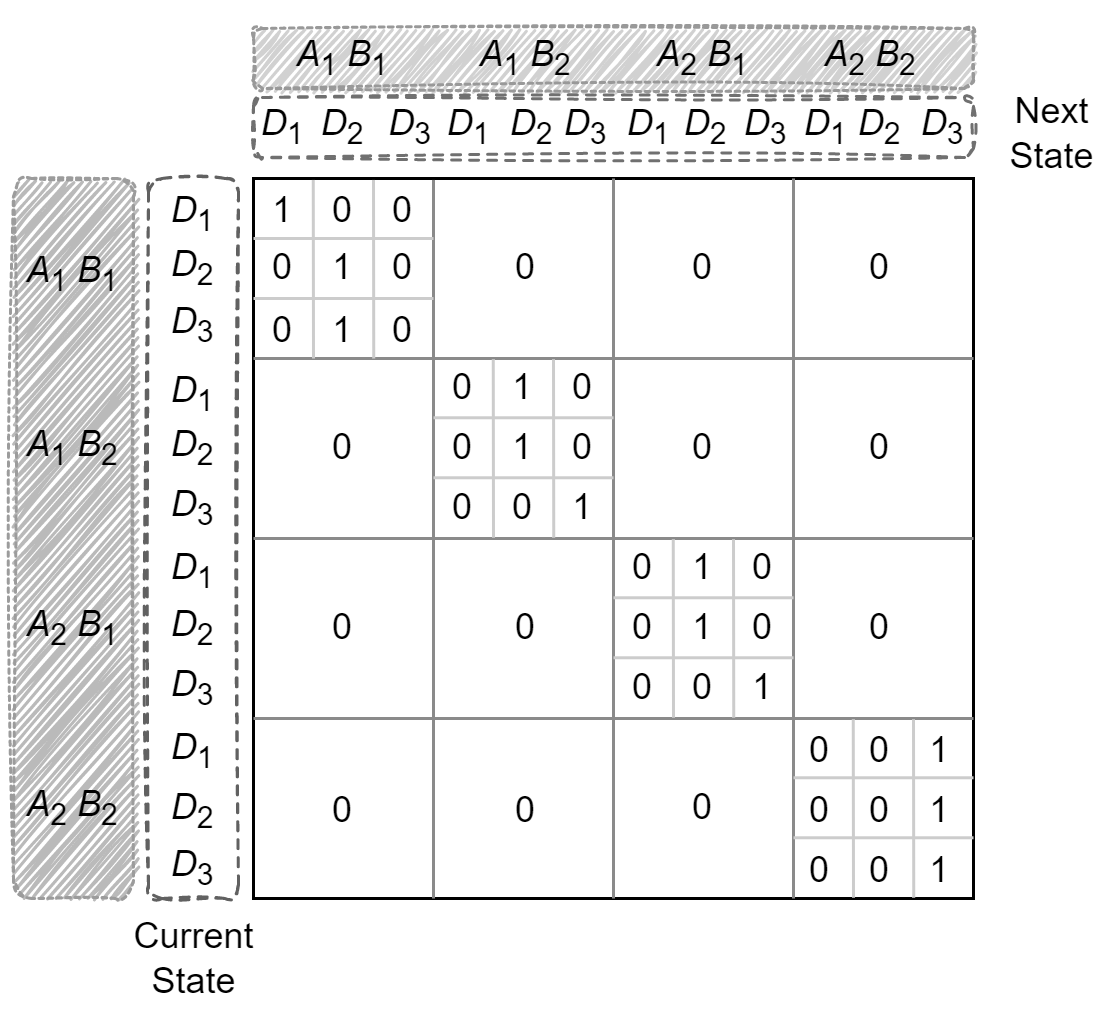
\includegraphics[width=0.65\linewidth]{Figures/transMatDiscrete.png}
	\caption[Transition matrix, $\underline{\underline{\mathbb{P}_{\tau}}}$ for discrete case]{Transition matrix, $\underline{\underline{\mathbb{P}_{\tau}}}$ for discrete case\protect\footnotemark} 
	\label{transMatDisc}
\end{figure}
\footnotetext{The values included in both Figures \ref{beliefDisc}, \ref{transMatDisc} are arbitrary, for illustration purposes.}

To elaborate a bit further on the meaning of the entries in the transition matrix, the second row and second column are examined, as displayed in Figure \ref{transMatDiscV2}.

\begin{figure}[H]
    \centering
	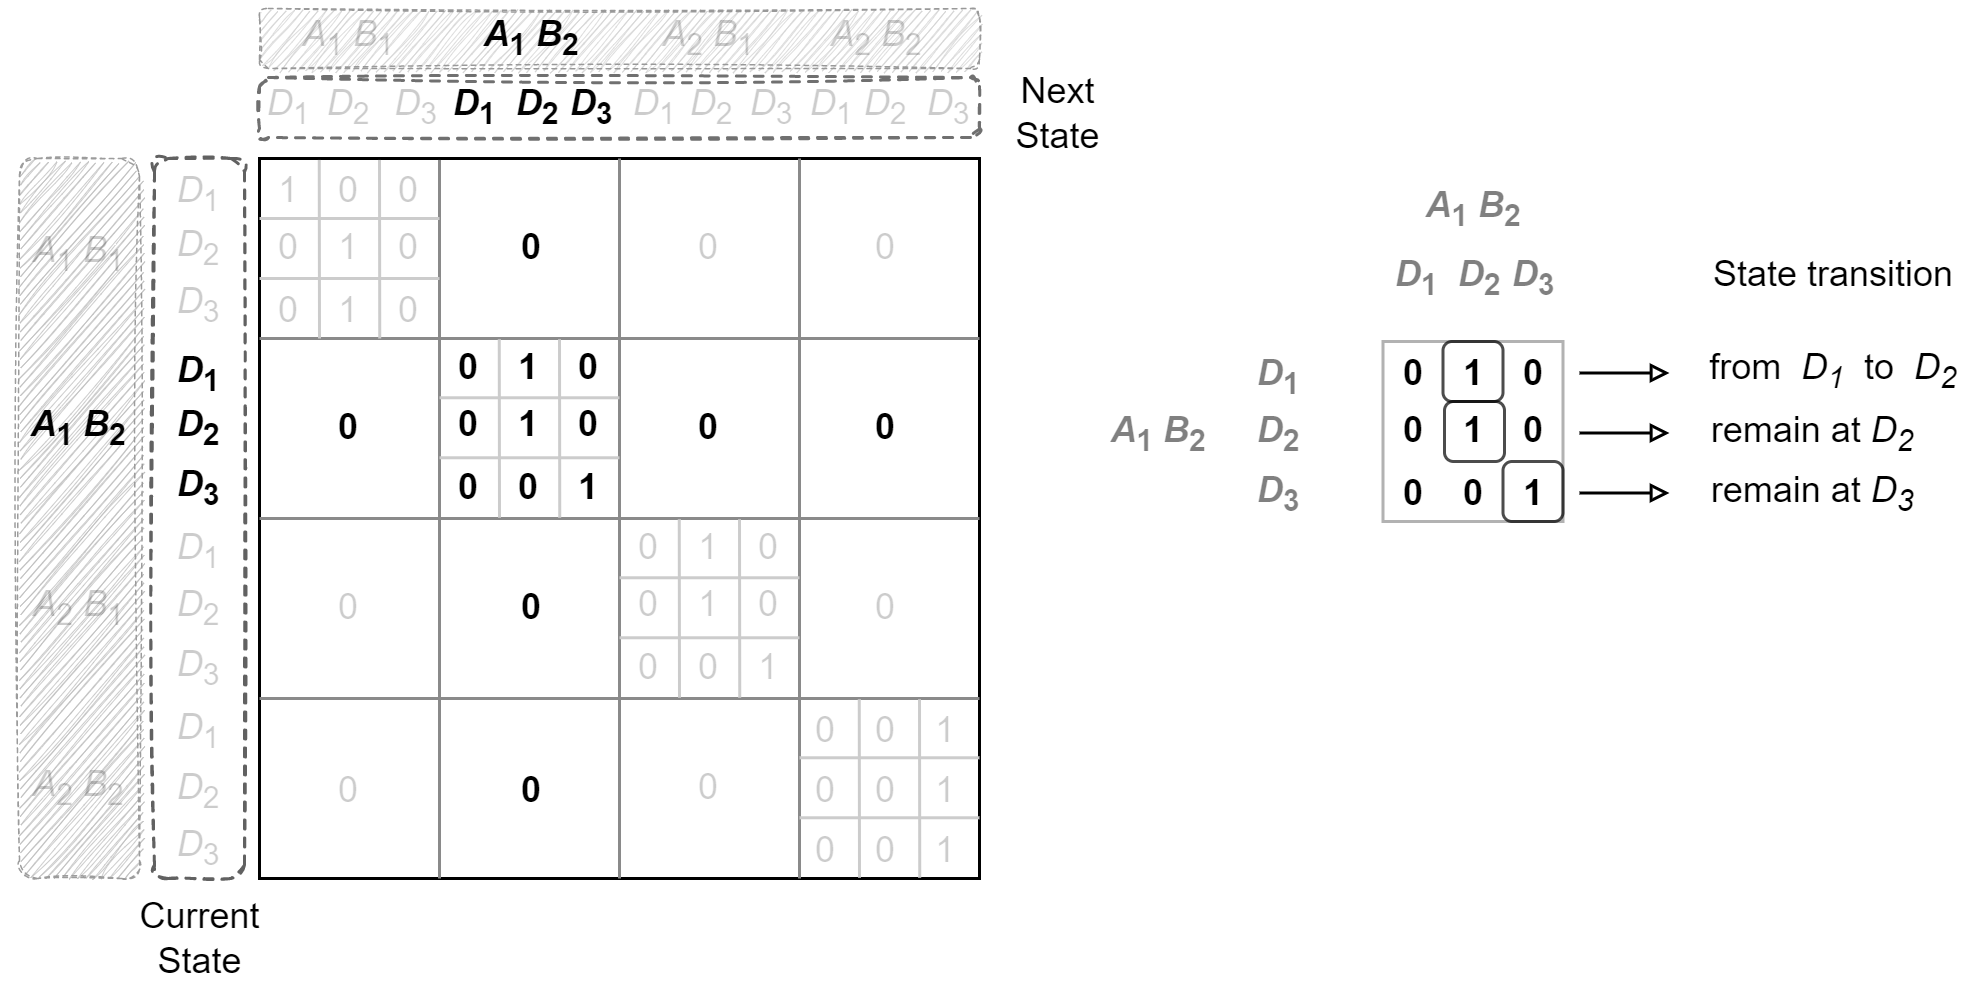
\includegraphics[width=\linewidth]{Figures/transMatFocus.png}
	\caption{Transition matrix, $\underline{\underline{\mathbb{P}_{\tau}}}$ for discrete case explanation} 
	\label{transMatDiscV2}
\end{figure}

In the examined part, knowing that the parameters $A, B$ have the values $A_1$ and $B_2$ respectively, the damage state will be $D_2$. This means that the agent can either shift from state $D_1$ to $D_2$, or remain to state $D_2$, or in the case the prior damage has already reached $D_3$, it can not go back in a less damaged state, so it will remain at $D_3$. It is observed that only the $3$ by $3$ sub-matrix that corresponds to the same $A, B$ values both in the row and the column indexing is populated with non-zero values, which is reasonable since the two parameters can not simultaneously be equal to different values. Lastly, an important property of the transition matrix is that each row needs to sum up to $1$ (as noted also for the belief vector).\\

% Further elaboration on the form of such a matrix are included in Appendix \ref{annexTransMat}.\\


Having defined the necessary quantities, the belief vector can be found using Bayes Theorem, applied in \glspl{POMDP}, avoiding time consuming sampling procedures like \gls{MCMC} or \gls{NUTS}. For a single entry of $b(s_{t+1})$ it holds:

\begin{equation}
    b(s_{t+1}) = \cfrac{p(o_{t+1}\mid s_{t+1})}{p(o_{t+1}\mid \underline{b})} \, \sum _{s_t\in \ccal{S}} p(s_{t+1}\mid s_t) \, b(s_t) \label{beliefOne}
\end{equation}

where the denominator is a normalizing constant, i.e. the so-called evidence in Bayes Theorem, which is equal to:

\begin{equation}
    p(o_{t+1}\mid \underline{b}) = \sum _{s_{t+1}\in \ccal{S}} p(o_{t+1}\mid s_{t+1}) \sum _{s_t\in \ccal{S}} p(s_{t+1}\mid s_t) b(s_t) \label{beliefNormConst}
\end{equation}

\newpage

Equations \ref{beliefOne}, \ref{beliefNormConst} can be generalized and rewritten in matrix notation:

\begin{equation}
    \underline{b}^{\prime} = \cfrac{\underline{\underline{\mathbb{O}}}(o_{t+1}) \odot \big[ \underline{\underline{\mathbb{P}}}^T\cdot \underline{b}\big]}{\Big [ \underline{\underline{\mathbb{O}}}^T(o_{t+1}) \cdot \big[ \underline{\underline{\mathbb{P}}}^T\cdot \underline{b}\big] \Big ]} \label{toyDiscEq}
\end{equation}

\blfootnote{The symbol $\odot$ in Equation \ref{toyDiscEq} denotes the Hadamar product, i.e. an elementwise matrix multiplication.}

As far as the \gls{DRL} aspect is concerned, apart from the belief vector, $\underline{b}$, the exposure time of the component, in other words the deterioration rate $\tau$, needs to be fed into the \gls{DNN}, since the current case constitutes a time dependent problem. A time parameter is a necessary input for the \gls{DNN} in order to define accurately the rate with which the system deteriorates at every given state, after any maintenance action.\\

To be more precise, for \gls{DDQN}, the belief vector $\underline{b}$ and the deterioration rate $\tau$ are passed as input to the \gls{DNN}, and after a forward pass the network yields the action-state value function for each action, $Q(s_t, a_i)$ for $i=1,2,3$, which is interpreted as the reward of taking a specific action $a_i$ given a state $s_t$. These three value functions constitute the knowledge based on which the agent will act, i.e. if the agent chooses to exploit what it already knows, the action with the highest $Q$-value (as derived from the \gls{DNN}) will be chosen. A schematic representation of the described \gls{DNN} architecture is displayed in Figure \ref{dnnToyDiscDDQN}.

\begin{figure}[H]
    \centering
	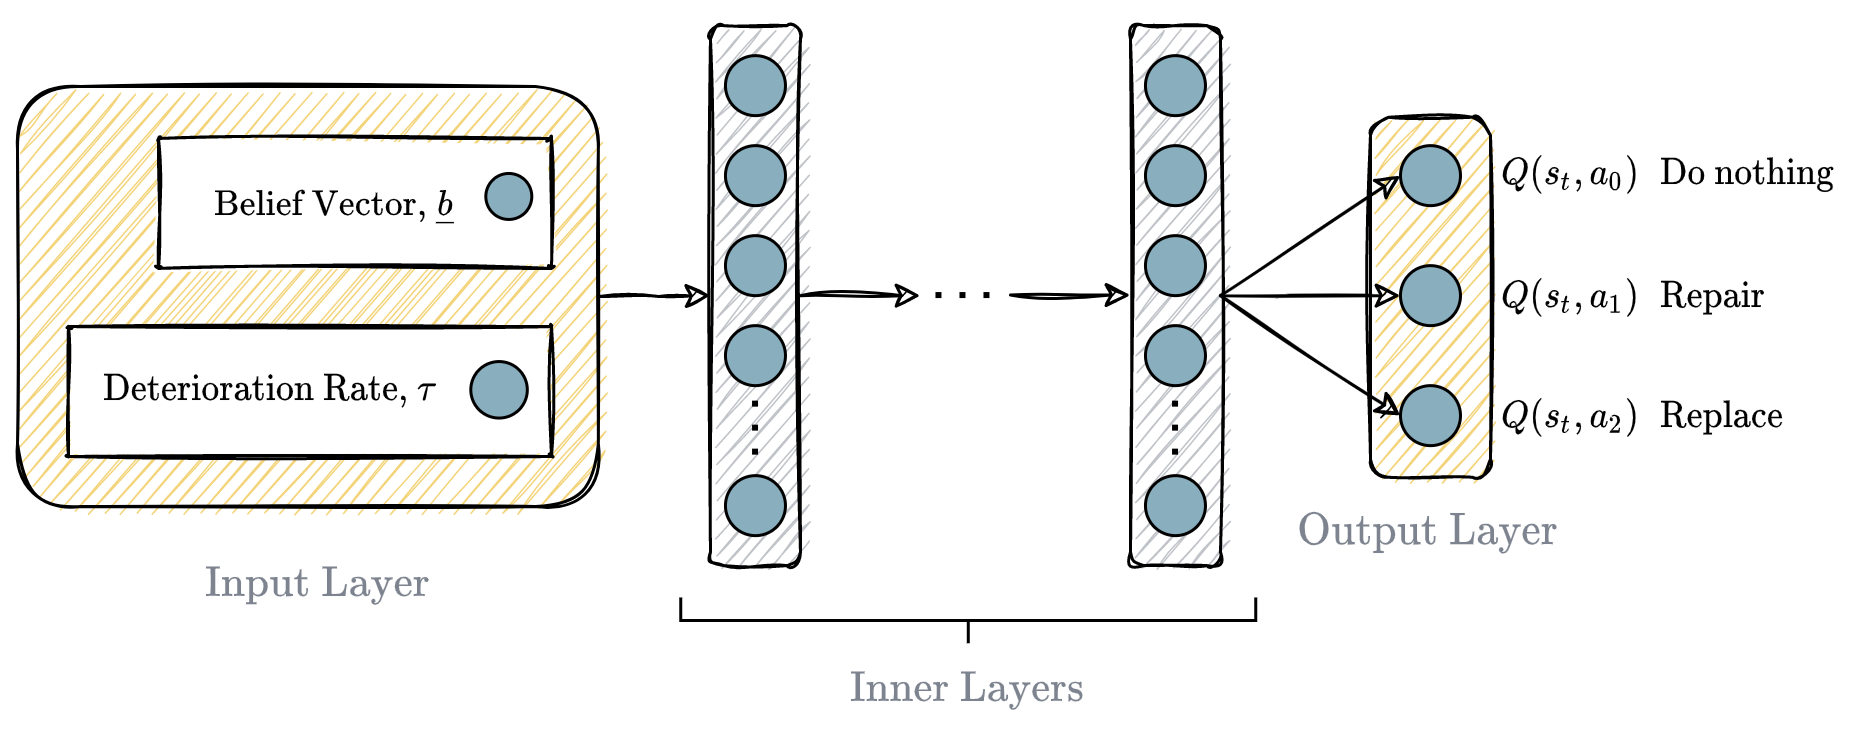
\includegraphics[width=\linewidth]{Figures/dnnToyDiscDDQN.png}
	\caption{\gls{DDQN} \gls{DNN} architecture for the discrete toy problem}
	\label{dnnToyDiscDDQN}
\end{figure}

When it comes to \gls{A2C} and \gls{PPO}, which are actor-critic algorithms, the same input, $\underline{b}$ and $\tau$, are passed to two different networks, namely the Actor and the Critic network. A forward pass of the former will yield directly the policy $\pi _{\theta}(a_i \mid s_t)$, i.e. the probability of choosing each action $a_i$ when being at state $s_t$, while the latter one returns the state value function $V_{\phi}(s_t)$, which corresponds to the reward of being at the state $s_t$ regardless from the chosen action. The aforementioned networks are depicted in Figure \ref{dnnToyDiscPPO}.

\begin{figure}[H]
    \centering
	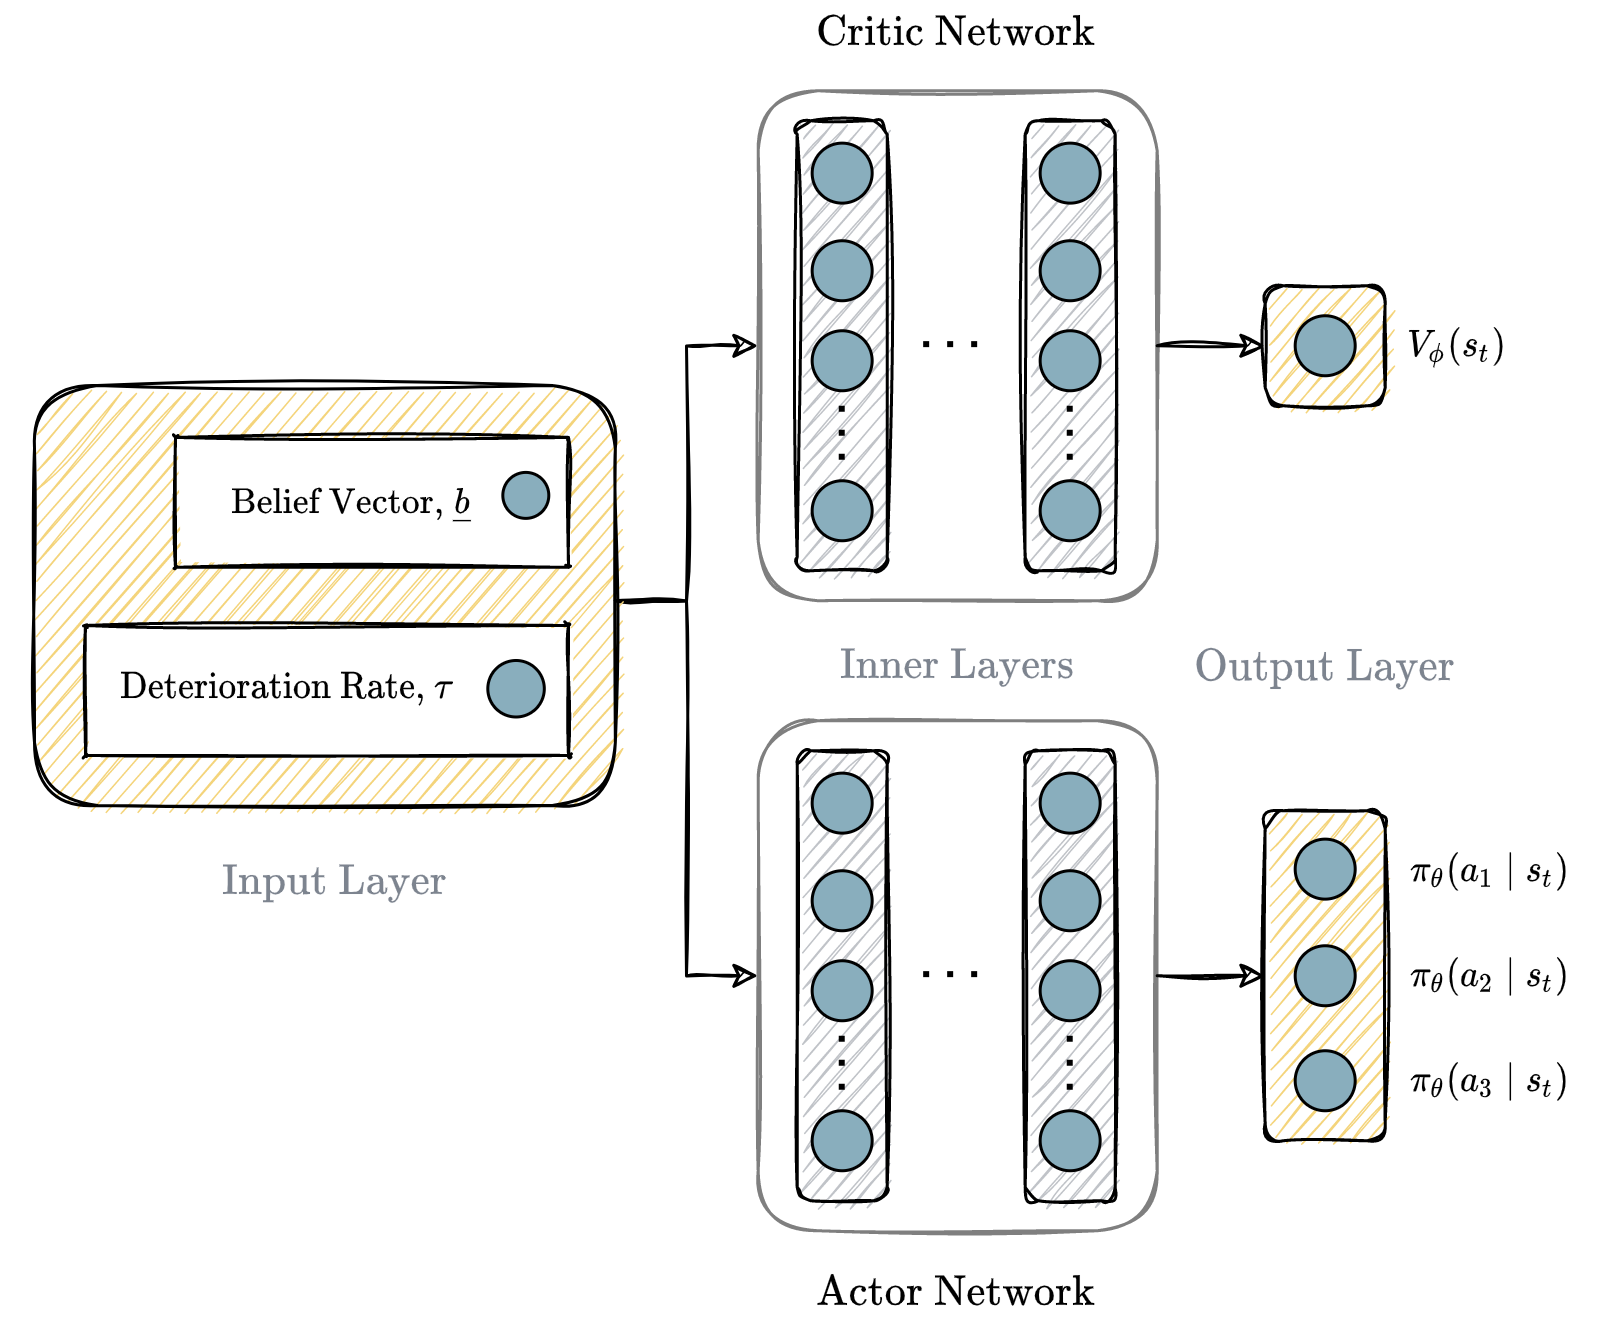
\includegraphics[width=0.9\linewidth]{Figures/dnnToyDiscPPO.png}
	\caption{Actor-critic \gls{DNN} architecture for the discrete toy problem}
	\label{dnnToyDiscPPO}
\end{figure}

It should be noted that although three algorithms were initially chosen to be tested, namely \gls{DDQN}, \gls{A2C} and \gls{PPO}, only two of them actually performed adequately. In particular, \gls{A2C} failed to yield optimal solutions both for the discrete and the continuous variations of the toy problem. Therefore, the necessary steps of the proposed framework regarding the remaining two algorithms are listed in Algorithms \ref{DDQNtoyDisc} and \ref{PPOtoyDisc} for \gls{DDQN} and \gls{PPO} respectively.\\

\newpage

To produce more compact and readable algorithms, several counting parameters are defined, which are explained in Tables \ref{ddqnCounts}, \ref{ppoCounts}, for \gls{DDQN} and \gls{PPO} respectively. 

\begin{table}[H]
    \centering
    \caption{Counters used for \gls{DDQN}}
    \label{ddqnCounts}
    \begin{tabular}{ccc}
        \toprule
        \textbf{Parameter} & \textbf{Name} & \textbf{Description} \\ \midrule
        $T$ & steps per episode & \begin{tabular}[c]{@{}c@{}}The amount of decision steps\\ considered for the maintenance\\ of the \gls{SDOF} system\end{tabular} \\ \midrule
        $T_{\text{update}}$ & target network update & \begin{tabular}[c]{@{}c@{}}Every how many steps the parameters\\ of the current neural network are\\ passed to the target one\end{tabular} \\ \midrule
        $M$ & number of episodes & \begin{tabular}[c]{@{}c@{}}The number of episodes employed\\ to train the \gls{DDQN} agent. Each \\episode consists of $T$ decision steps\end{tabular}\\ \bottomrule
    \end{tabular}
\end{table}

\vspace{1cm}

\begin{table}[H]
    \centering
    \caption{Counters used for \gls{PPO}}
    \label{ppoCounts}
    \begin{tabular}{ccc}
        \toprule
        \textbf{Parameter} & \textbf{Name} & \textbf{Description} \\ \midrule
        $T$ & steps per episode & \begin{tabular}[c]{@{}c@{}}The amount of decision steps\\ considered for the maintenance\\ of the \gls{SDOF} system\end{tabular} \\ \midrule
        $N$ & steps per epoch & \begin{tabular}[c]{@{}c@{}}The amount of decision steps\\ employed for a single batch \\ training of the \gls{PPO} agent\end{tabular} \\ \midrule
        $M$ & number of epochs & \begin{tabular}[c]{@{}c@{}}The number of epochs used to\\ train the \gls{PPO} agent in total. Each\\ epoch consists of $N$ decision steps\end{tabular}\\ \bottomrule
    \end{tabular}
\end{table}

\begin{algorithm}[H]
    \caption{\acrfull{DDQN} - Discrete Toy Problem}
    \label{DDQNtoyDisc}
    \SetKwProg{epsGreedy}{Choose Action}{:}{}
    Initialize primary network weights $\theta$\\
    Initialize target network weights $\theta^{-}$\\
    Initialize replay buffer\\
    \For {$episode \gets 1$ \KwTo $M$}{
        $s_t \gets$ reset environment \tcp{$\tau \gets 0$, initialize belief vector $\underline{b}$ to zero damage}\\
        \For {$t \gets 1$ \KwTo $T$}{
            $\tau \gets \tau + 1$\\
            Calculate the next belief vector according to\\
            $ \underline{b}^{\prime} = \cfrac{\underline{\underline{\mathbb{O}}}(o_{t+1}) \odot \big[ \underline{\underline{\mathbb{P}}}^T\cdot \underline{b}\big]}{\Big [ \underline{\underline{\mathbb{O}}}^T(o_{t+1}) \cdot \big[ \underline{\underline{\mathbb{P}}}^T\cdot \underline{b}\big] \Big ]} $ \tcp{the transition matrix $\underline{\underline{\mathbb{P}}}$ depends on $\tau$} \\
            \epsGreedy{according to $\epsilon$-greedy method}{
            Generate random number $rand \in [ 0,1 ] $\\
            \If{$rand<\epsilon$}{Sample a random action, $a_t \in \ccal{A}$ \tcp{Explore}}
            \Else{$a_t = \underset{a_t\in \ccal{A}}{\text{argmax}} Q(s_t, a_t)$ \tcp{Exploit}}
            }
            \If{$a_t$ is ``replace''}{
                $\tau \gets 0$
            }
            \ElseIf{$a_t$ is ``repair''}{
                $\tau \gets \text{max}(\tau - 2, 0)$
            }
            Calculate $P_f$ for the belief vector $\underline{b}^{\prime}$\\
            $R(s_t, a_t) \gets C_{a_t} + P_f \, C_{\text{F}}$\\
            Store tuple $\left( s_t, a_t, R(s_t,a_t), s_{t+1} \right)$ in replay buffer \tcp{$s_t = \langle \underline{b}, \tau \rangle$, $s_{t+1} = \langle \underline{b}^{\prime}, \tau \rangle$}\\
            $s_t \gets s_{t+1}$\\
            Sample batch of tuples $\left( s_i, a_i, R(s_i,a_i), s_{i+1} \right)$ from replay buffer\\
            \If{$s_{i+1}$ is terminal state}{$y_i = R(s_i, a_i)$}
            \Else{$y_{t}=R(s_{t}, a_{t})+\gamma \,Q\left(s_{t+1}, \arg \max Q\left(s_{t+1}, a_{t+1} \mid \theta \right) \mid \theta^- \right)$}
            Update parameters $\theta$ according to: $\nabla_{\theta} L\left(\theta \right) \simeq \sum \left[\left( Q\left(s_i, a_i \mid \theta \right) -y_i \right) \nabla_{\theta} Q\left(s_i, a_i \mid \theta \right)\right]$\\
            \If{$T_{\text{update}}$}{$\theta ^- = \theta$} 
        }
    }
\end{algorithm}


\begin{algorithm}[H]
    \caption{\acrfull{PPO} - Discrete Toy Problem}
    \label{PPOtoyDisc}
    \SetKw{actor}{Actor Net}
    \SetKw{ppoTrain}{Train Agent}
    \SetKw{critic}{Critic Net}
    \SetKw{or}{or}
    Initialize policy (actor) network weights $\theta$\\
    Initialize value function (critic) network weights $\phi$\\
    \For {$episode \gets 1$ \KwTo $M$}{
        $s_t \gets$ reset environment \tcp{$t \gets 0, \, \tau \gets 0$, initialize belief vector $\underline{b}$ to zero damage}\\
        \For {$n \gets 1$ \KwTo $N$}{
            $t \gets t + 1, \, \tau \gets \tau + 1$\\
            Calculate the next belief vector according to\\
            $ \underline{b}^{\prime} = \cfrac{\underline{\underline{\mathbb{O}}}(o_{t+1}) \odot \big[ \underline{\underline{\mathbb{P}}}^T\cdot \underline{b}\big]}{\Big [ \underline{\underline{\mathbb{O}}}^T(o_{t+1}) \cdot \big[ \underline{\underline{\mathbb{P}}}^T\cdot \underline{b}\big] \Big ]} $ \tcp{the transition matrix $\underline{\underline{\mathbb{P}}}$ depends on $\tau$} \\
            $\pi _{\theta} (a_t \mid s_t) \gets $ \actor ($s_t$) \tcp{forward pass of the actor network}\\
            $V_{\phi}(s_t) \gets $ \critic ($s_t$) \tcp{forward pass of the critic network}\\
            $a_t \gets$ sample $\pi _{\theta} (a_t \mid s_t)$\\
            \If{$a_t$ is ``replace''}{
                $\tau \gets 0$
            }
            \ElseIf{$a_t$ is ``repair''}{
                $\tau \gets \text{max}(\tau - 2, 0)$
            }
            Calculate $P_f$ for the belief vector $\underline{b}^{\prime}$\\
            $R(s_t, a_t) \gets C_{a_t} + P_f \, C_{\text{F}}$\\
            Store tuple $\left( s_t, a_t, \pi _{\theta} (a_t \mid s_t), V_{\phi}(s_t), R(s_t,a_t) \right)$ in $\ccal{D}_k$ \tcp{$s_t = \langle \underline{b}, \tau \rangle$}\\
            $s_t \gets s_{t+1}$ \tcp{$s_{t+1} = \langle \underline{b}^{\prime}, \tau \rangle$}\\
            \If{$t=T$ \or $n=N$}{
                \If{$t=T$}{
                    $V_{\phi}(s_{t+1}) \gets 0$\\
                    $s_t \gets$ reset environment \tcp{$t \gets 0, \, \tau \gets 0$, initialize belief vector $\underline{b}$ to zero damage}
                }
                \Else{
                    $V_{\phi}(s_{t+1}) \gets \critic (s_t)$
                }
                Returns $\delta _t \gets R(s_t, a_t) + \gamma \, V_{\phi}(s_{t+1}) - V_{\phi}(s_t)$\\
                Advantages $A_t \gets \delta _t + (\gamma \, \lambda ) \, \delta_{t+1} + \ldots + (\gamma \, \lambda ) ^{T-t+1} \delta _{T-1}$\\
                Store $\delta _t, A_t$ in $\ccal{D}_k$
            }
        }
        \ppoTrain($\ccal{D}_k$)
    }
\end{algorithm}

\newpage

The function ``\textit{Train Agent}'' is further elaborated in Algorithm \ref{PPOtrainAgentToy}.\\

\begin{algorithm}
    \caption{\acrfull{PPO} agent training - Toy problem}
    \label{PPOtrainAgentToy}
    \SetKwProg{ppoTrain}{Train Agent}{:}{}
    \ppoTrain{($\ccal{D}_k$)}{
            Update parameters $\phi$, using the Critic cost function:
            $$L^{\text{VF}}(\phi) = \sum_{t=1}^{T} \left ( V_{\phi}(s_t)-\delta_t \right ) ^2 $$\\
            Update parameters $\theta$, using the Actor loss function:
            $$L^{\text{CLIP}}(\theta) = \sum_{t=1}^{T} \min \left(\cfrac{\pi_{\theta}\left(a_{t} \mid s_{t}\right)}{\pi_{\theta_{\text{old}}}\left(a_{t} \mid s_{t}\right)} A_t \left(s_{t}, a_{t}\right), \, \text{clip} \left( \cfrac{\pi_{\theta} \left( a_{t} \mid s_{t} \right )}{\pi_{\theta_{\text{old}}} \left( a_{t} \mid s_{t} \right )}, 1-\varepsilon, 1+\varepsilon \right) A_t \right)$$
            via minibatch stochastic gradient ascent with Adam
        }
\end{algorithm}

\vspace{0.5cm}

%------------------------------------------------------------------------------
%	CONTINUOUS CASE
%------------------------------------------------------------------------------


\subsubsection{Continuous case} \label{toyDiscSec}

Following the discrete case, the stochastic parameters $A$ and $B$ are now considered to be continuous variables. The assumed prior distributions are displayed in Table \ref{deterParams}.

\begin{table}[H]
    \centering
    \caption{Parameters of the stochastic deterioration model}
    \label{deterParams}
    \begin{tabular}{cccc}
        \toprule
        \textbf{Parameter} & \textbf{Distribution} & \textbf{Mean} & \textbf{\gls{CV}} \\ \midrule
        $A$ & Lognormal & $8.0E-03$ & $0.5$ \\
        $B$ & Normal & $1.5$ & $0.3$ \\ \bottomrule
    \end{tabular}
\end{table}

\newgeometry{,hmargin=3cm,vmargin=3cm,landscape}
\savegeometry{landscape}

Since the continuous case of the toy problem does not impose any simplification as far as the proposed framework is concerned, the already presented flowchart (Figure \ref{genFlow}) is now being updated and elaborated further, and is depicted in Figure \ref{flowToy}.

\vspace{1cm}

\begin{figure}[H]
    \centering
	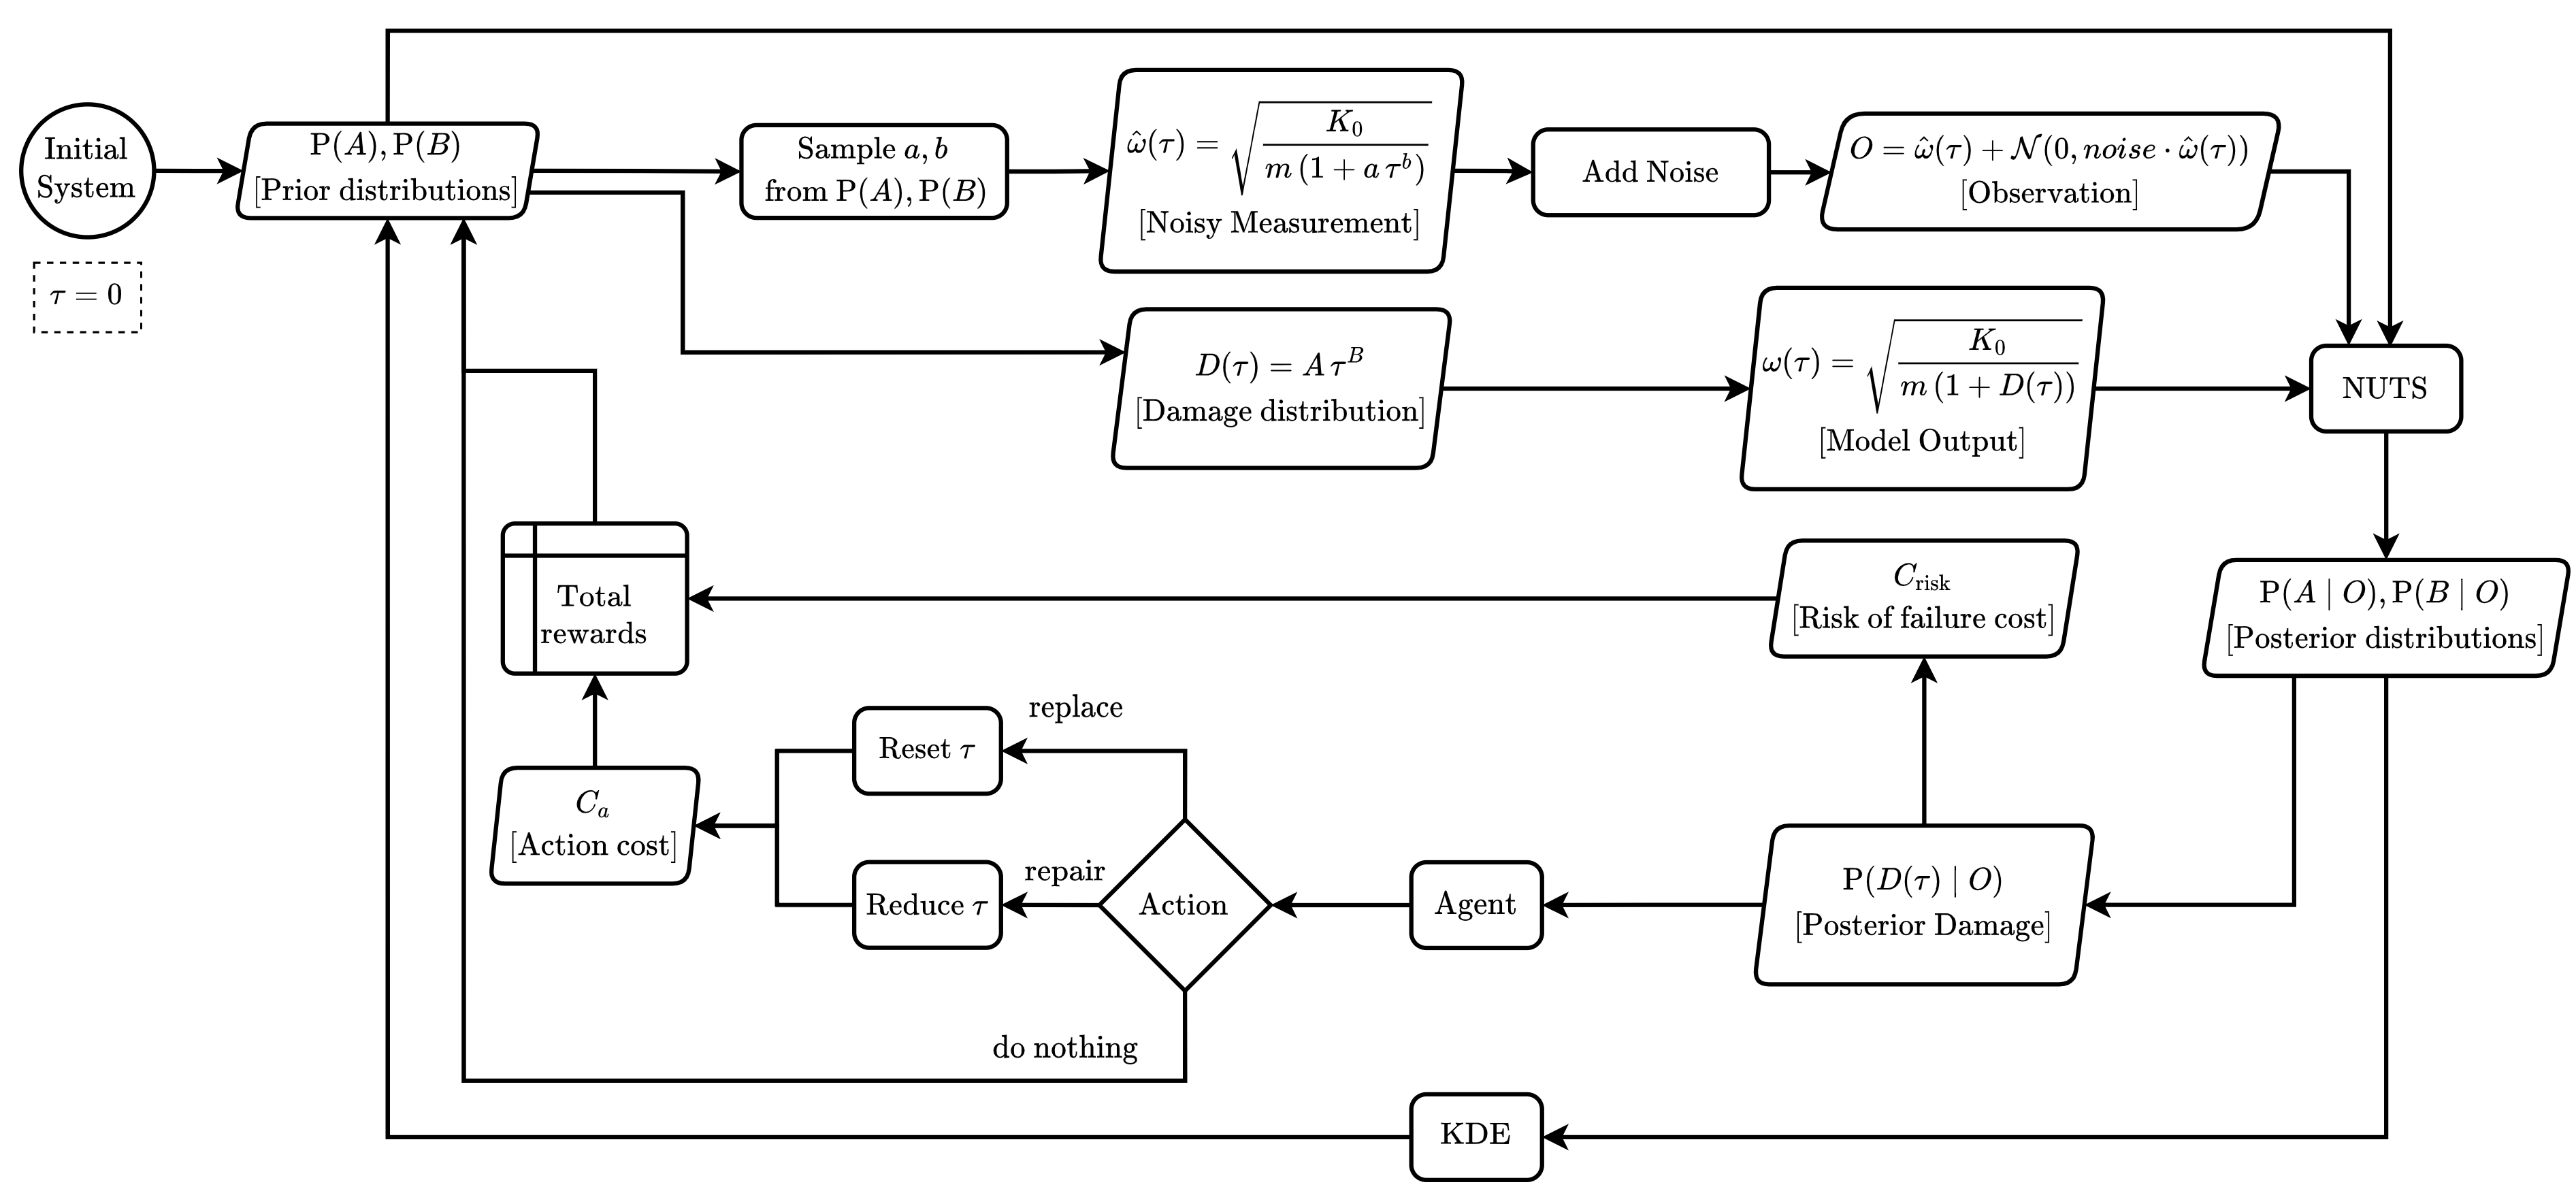
\includegraphics[width=\linewidth]{Figures/toyFlow.png}
	\caption{Framework flowchart for the toy problem}
	\label{flowToy}
\end{figure}

\restoregeometry

As displayed above, the parameters of interest that will be updated in every iteration are the distributions of $A, B$, hence, $\prob{A}, \prob{B}$, which are used as priors for the Bayesian inference. These distributions are used both to define the damage distribution $D(\tau) = A\, \tau ^B$, and to create the noisy measurement based on sampled $a, b$ values. The measurement will be further contaminated with noise, as seen at the top part of the flowchart, while the damage distribution is used to compute the model output:

$$ \omega = \sqrt{\cfrac{K_0}{m\big( 1 + D(\tau)\big)}}$$

Then, the observation, the model output and the prior distribution are passed to the \gls{NUTS} algorithm to yield the posterior distributions of $A, B$ and subsequently $D(\tau)$. These posterior distributions, $\prob{A \mid O}, \prob{B \mid O}$ are transformed into priors using a \gls{KDE} scheme. The updated damage distribution $\prob{D(\tau) \mid O}$ is used to calculate the risk of failure cost $C_{\text{risk}}$ which is added to the stored total reward of the iteration, but it is also passed to the agent in order to choose an action based on it. If the agent chooses to perform a maintenance action, this would result to a modification of the deterioration rate while yielding also an additional action cost $C_a$ which is added as well to the stored total reward. Before proceeding to the next iteration, the deterioration rate will be incremented by $1$. This loop is being ran for $20$ decision steps, and the quantity that needs to be optimized, i.e. minimized, is the total reward, thus the total maintenance cost.\\

A detailed description of the parameter updating procedure is presented in Algorithm \ref{bmuToy}.\\

% As displayed above, the parameters of interest that will be updated in every iteration are $\underbar{\theta} = \langle A, B, D(\tau) \rangle$. It is worth being mentioned that, although $D(\tau)$ is included in the system parameters, $\underbar{\theta}$, its distribution can be derived deterministically by drawing samples from the distributions of $A$ and $B$. This is the reason why in the drawn flowchart only the posterior distributions are acting as input (priors) for the next iteration, and not the possibly altered distribution of $D(\tau)$. On a more technical note, since the posteriors are not available in a closed-form, but they are shaped through an adequate number of samples, the priors for the following decision step are being derived using \gls{KDE}. 

% The observation is denoted as $\underbar{O} = \langle \omega \rangle$ and represents the noisy measurement that has been passed through the \gls{OMA} scheme, that itself contributed with additional noise.\\

\begin{algorithm}[H]
    \caption{Deterioration model parameters updating - Toy Problem}
    \algorithmfootnote{This algorithm focuses only on the Bayesian inference and the updating of the parameters. This is why the action part is covered abstractly.}
    \label{bmuToy}
    \SetKwProg{Procedure}{DeteriorationParametersUpdating}{:}{}
    \SetKwProg{nuts}{\gls{NUTS}}{:}{}
    \Procedure{( $\prob{A}, \prob{B}, mass, K_0, noise, T$ )}{
    $D(0) \gets 0$\\
    $\tau \gets 0$\\
    \For {$t\gets 1$ \KwTo $T$}{
        $\tau \gets \tau + 1$\\
        $\omega _0$ \gets $\sqrt{\cfrac{K_0}{mass\, \left( 1 + D(\tau) \right)}}$ \tcp{mean $\omega$}\\
        Generate $\omega_{\text{obs}} \gets \ccal{N}(\omega_0, noise)$\\
        \nuts{( $\prob{A}, \prob{B}, \omega_{\text{obs}}$ )}{
        \KwOut{$\prob{A \mid \omega_{\text{obs}}}, \prob{B \mid \omega_{\text{obs}}}, \prob{D(\tau)} $}}\\
        Choose action, $a_t$ \tcp{as explained in the \gls{DRL} algorithm}\\
        Adjust $D(\tau)$ distribution based on $a_t$\\
        Sample $A, B$ from $\prob{A \mid \omega_{\text{obs}}}, \prob{B \mid \omega_{\text{obs}}}$\\
        $D(\tau) \gets A\, \tau^B$ \tcp{will be used to calculate mean $\omega$}\\
        $\prob{A}, \prob{B} \gets \prob{A \mid \omega_{\text{obs}}}, \prob{B \mid \omega_{\text{obs}}}$ \tcp{posteriors become priors through \gls{KDE}}
        }
    }
\end{algorithm}

\vspace{1cm}

The first term of the total cost during an iteration is the already mentioned risk of failure cost, which is being computed as the product of the probability of failure times the cost of failure, $P_f \cdot C_{\text{fail}}$. The probability of failure, $P_f$ in the current simplified application is considered equal to the number of samples from the damage distribution that are located above the failure threshold, divided by the total number of samples (Figure \ref{failProb}).

\begin{figure}[H]
    \centering
	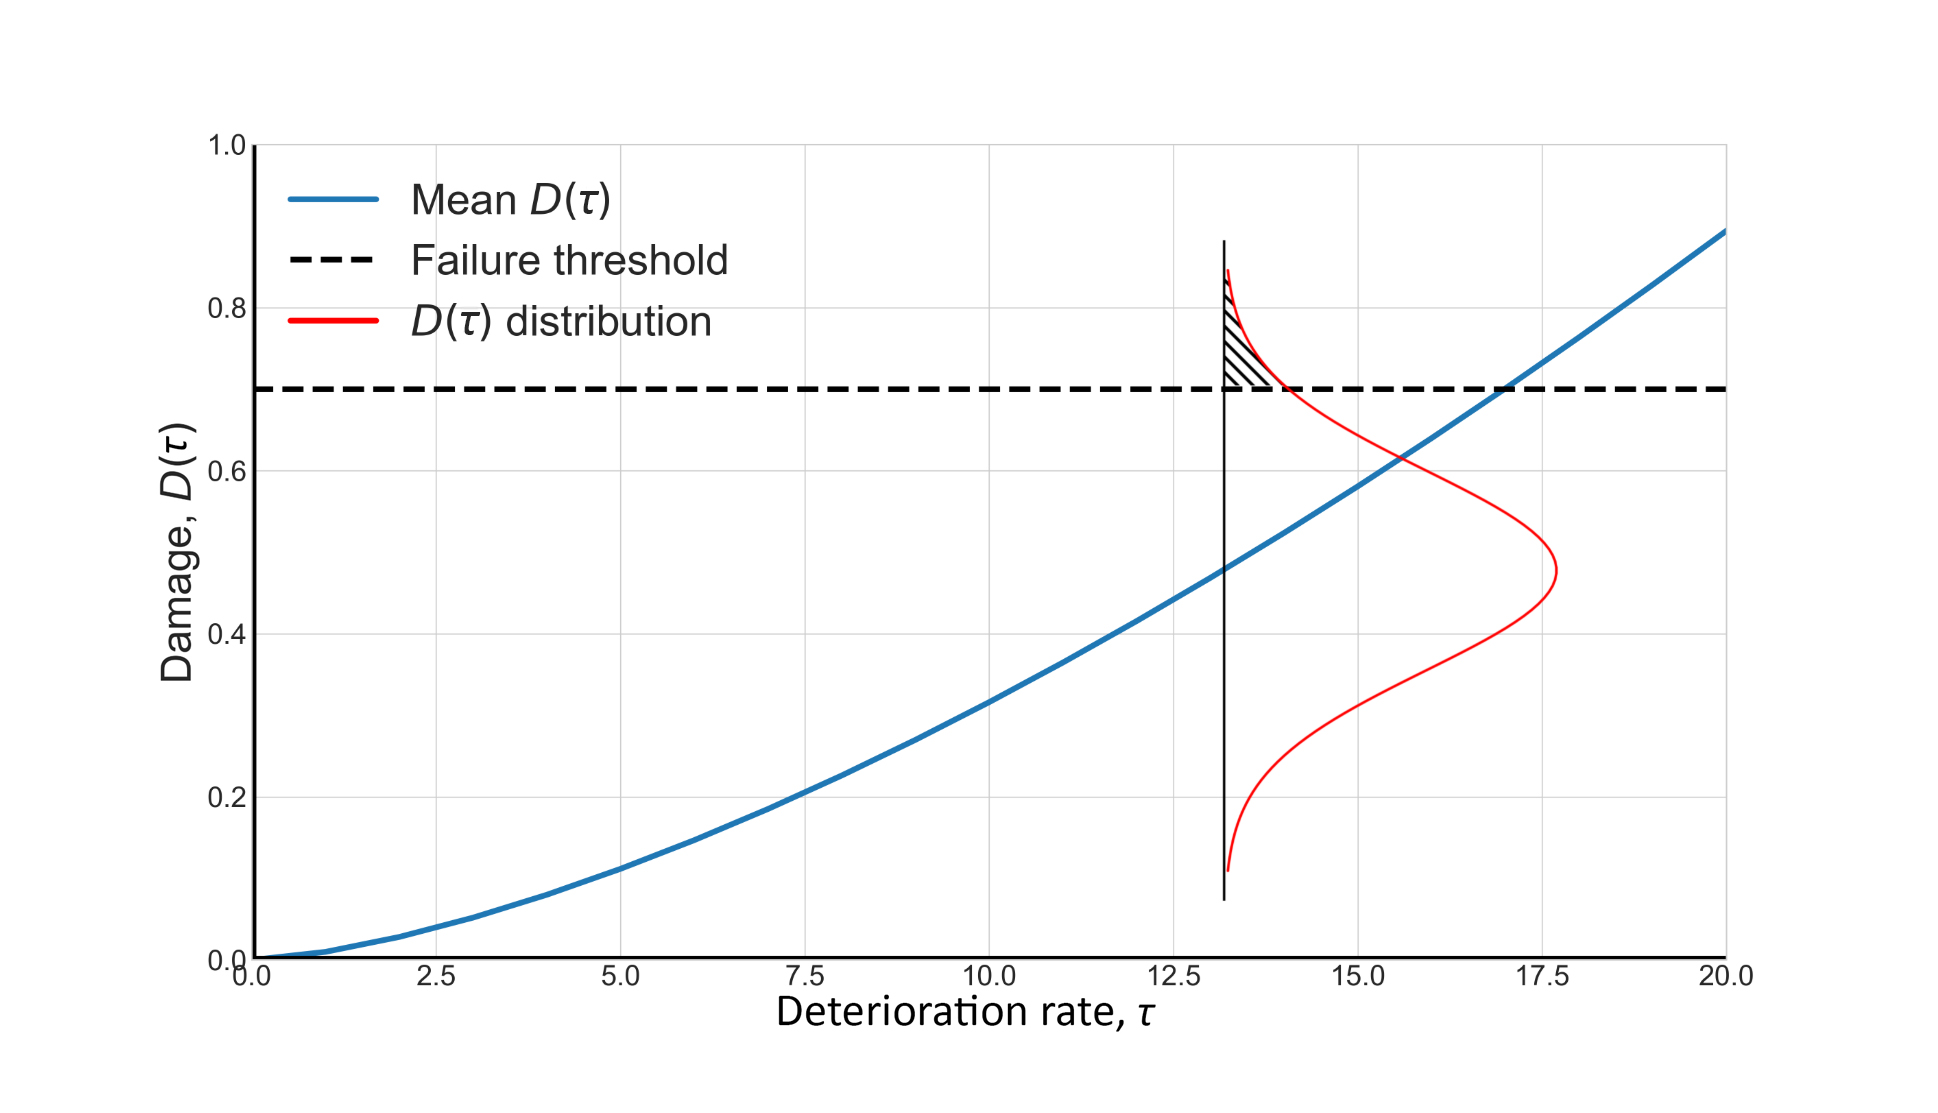
\includegraphics[width=0.85\linewidth]{Figures/failureProb.jpg}
	\caption[Failure Probability calculation]{Failure Probability calculation \protect\footnotemark}
	\label{failProb}
\end{figure}

\footnotetext{The curves (values and shape) illustrated in Figure \ref{failProb} are arbitrary, for explanatory reasons.}


Moving to the \gls{DRL} part of the framework, the need to select a discrete number of features that will accurately describe each deterioration state has emerged, and subsequently will be fed into the \gls{DNN}. For this purpose, the statistical moments of the $D(\tau)$ distribution were chosen, namely, the mean, the variance, the skewness and the kurtosis. As mentioned already for the discrete case, the examined problem is time dependent, meaning that the deterioration rate, $\tau$ of the structure needs also to be given as an input to the \gls{DNN}. Regarding the neurons in the output layer, they correspond to the action state value functions for the three different actions when using the \gls{DDQN} algorithm. The aforementioned characteristics of the \gls{DNN} architecture are demonstrated in Figure \ref{dnnToyContDDQN}.

\begin{figure}[H]
    \centering
	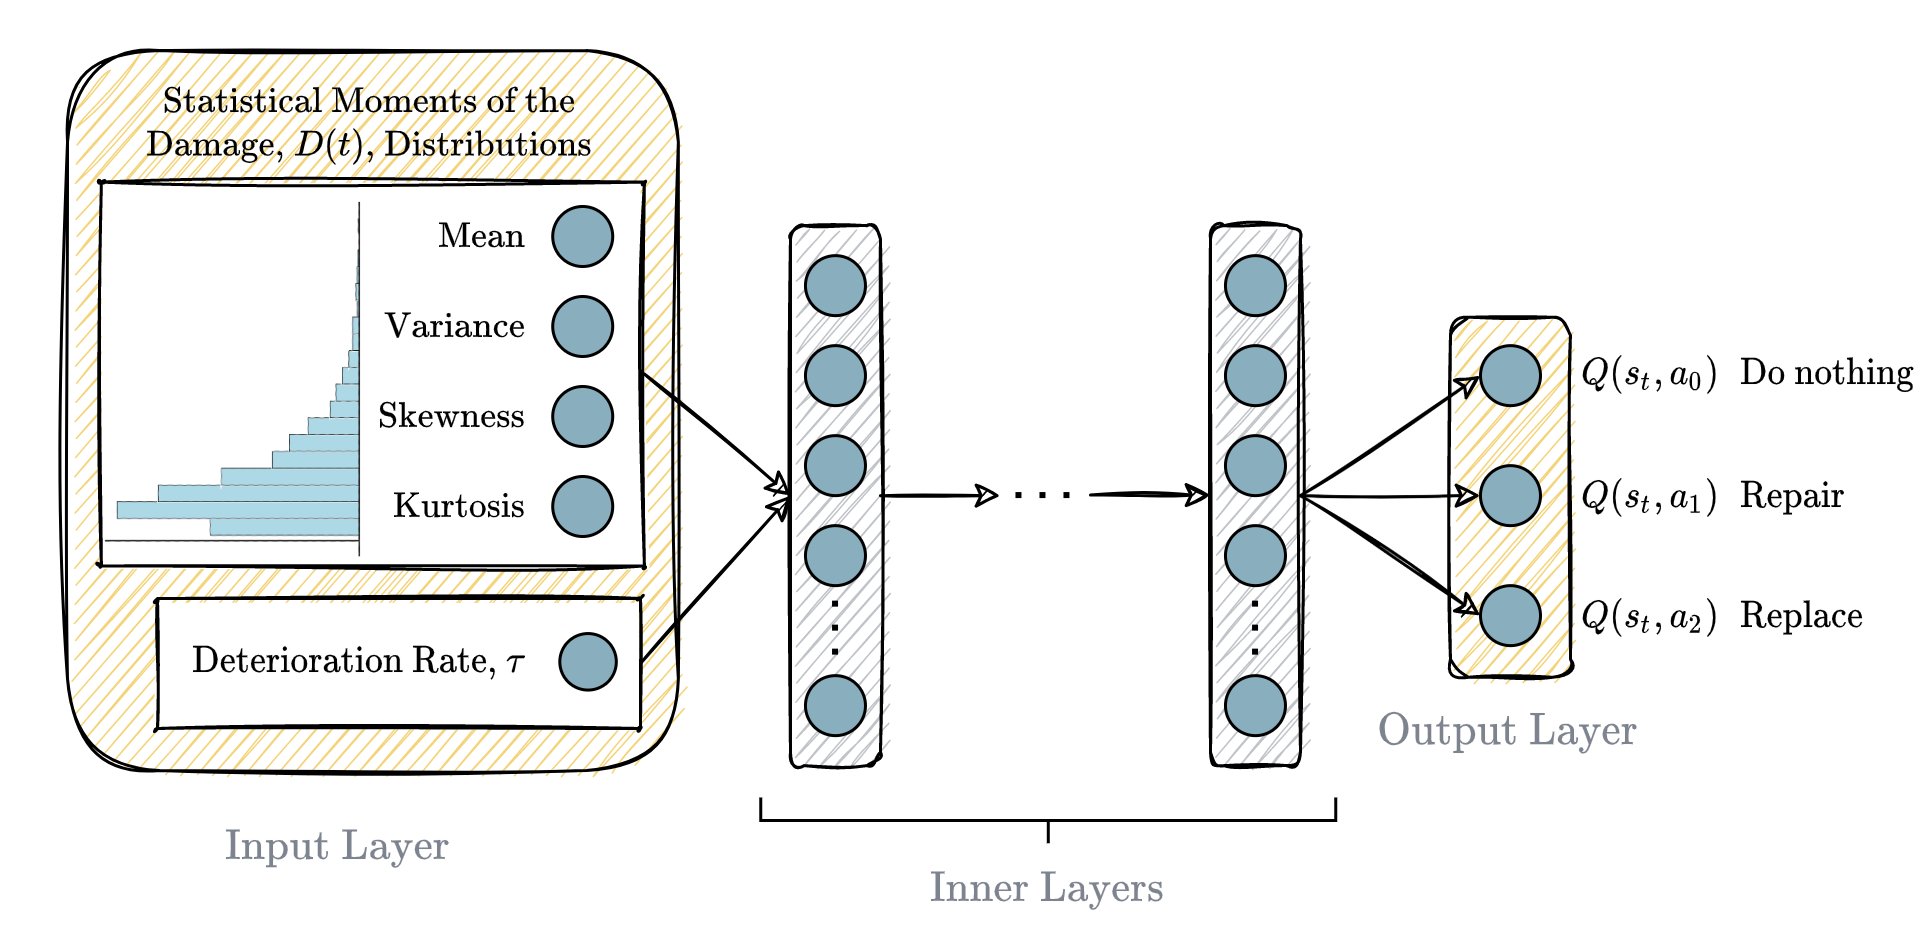
\includegraphics[width=\linewidth]{Figures/dnnToyContDDQN.png}
	\caption{\gls{DDQN} \gls{DNN} architecture for the continuous toy problem}
	\label{dnnToyContDDQN}
\end{figure}

Accordingly, for actor-critic algorithms, hence, also actor and critic \glspl{DNN}, the architecture is displayed in Figure \ref{dnnToyContPPO}.

\begin{figure}[H]
    \centering
	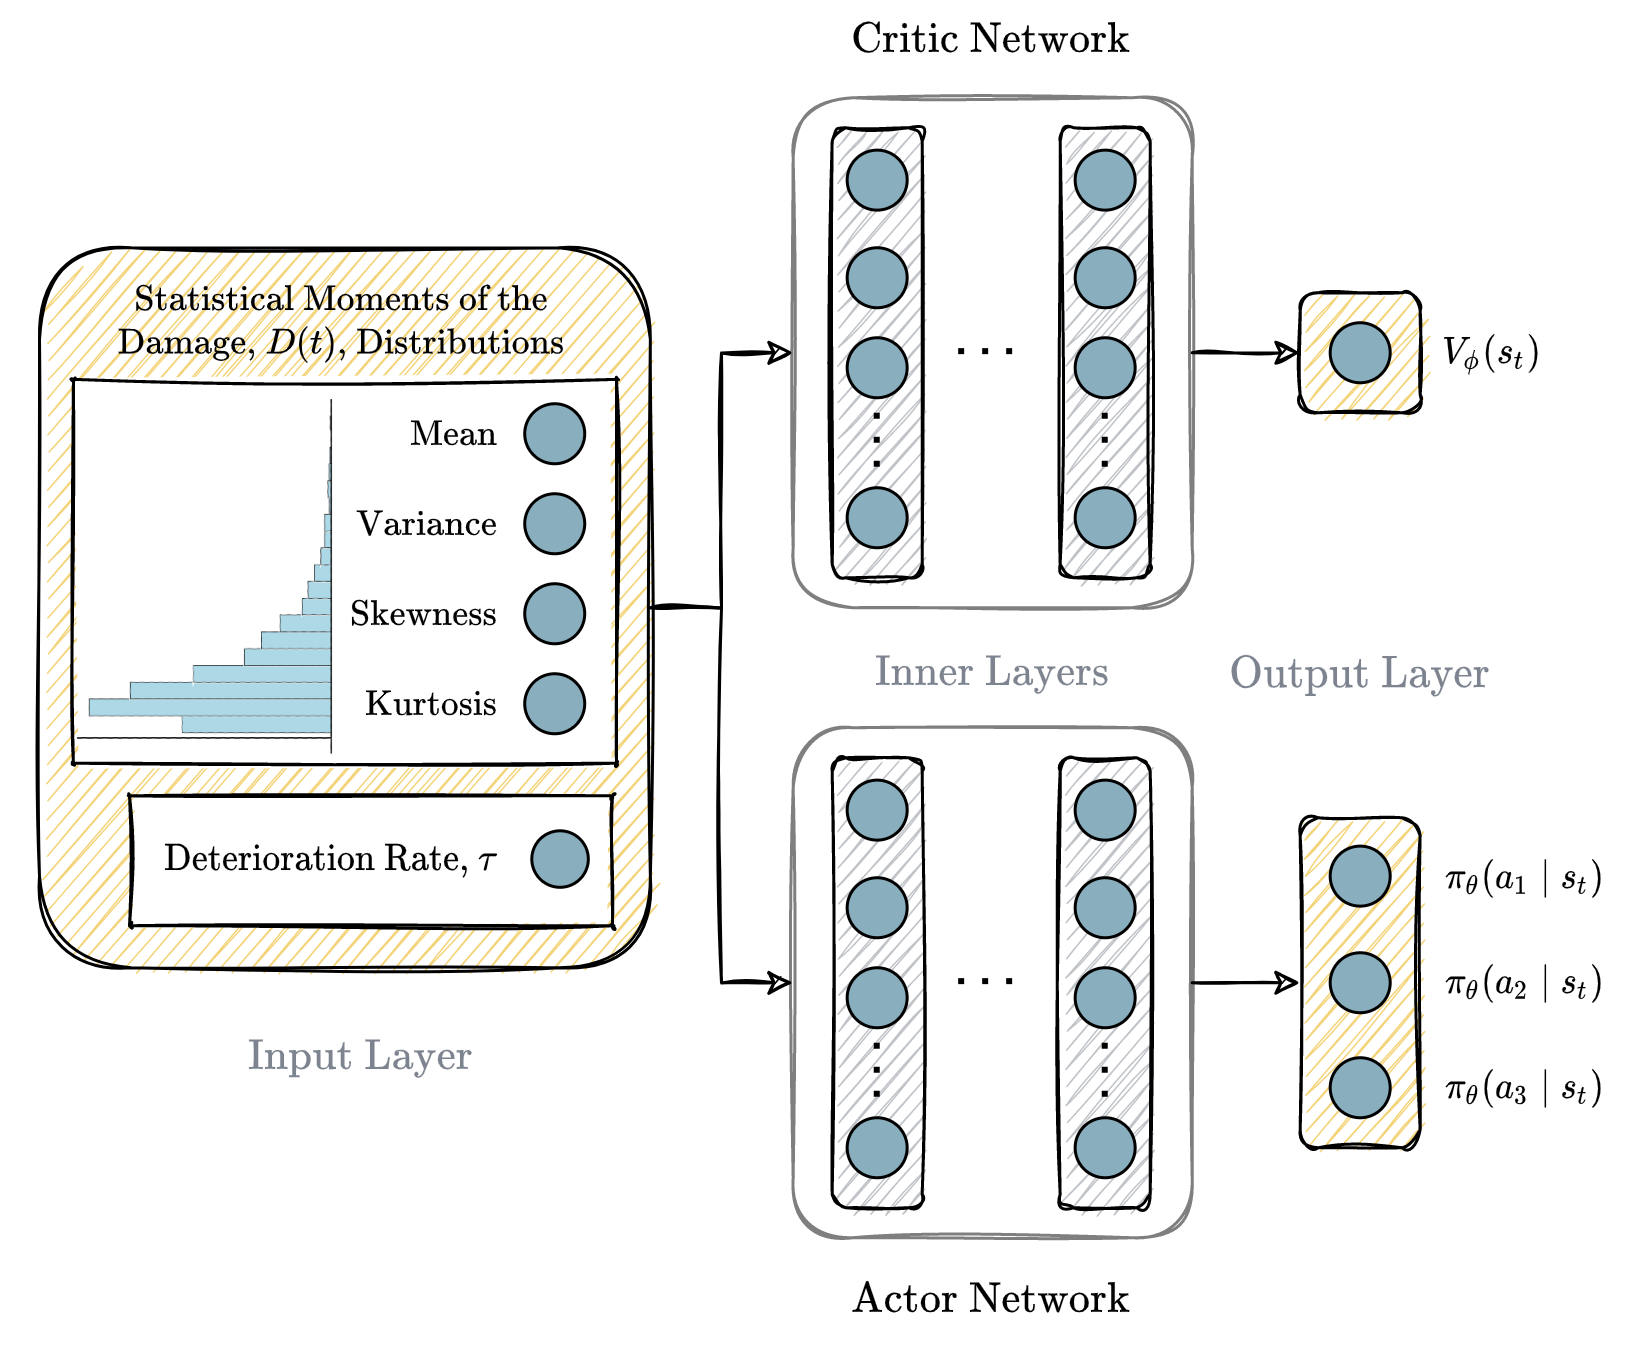
\includegraphics[width=0.9\linewidth]{Figures/dnnToyContPPO.png}
	\caption{Actor-critic \gls{DNN} architecture for the continuous toy problem}
	\label{dnnToyContPPO}
\end{figure}

It has already been mentioned that only two out of the three tried algorithms managed to produce valuable results, with \gls{A2C} being the one that under-delivered. Thus, the detailed procedure of the proposed framework concerning \gls{DDQN} and \gls{PPO} about the continuous variation of the toy problem, is presented in Algorithms \ref{DDQNtoy} and \ref{PPOtoy} respectively. As with the discrete version of the problem, the counters used in the coming algorithms are presented in Tables \ref{ddqnCounts} and \ref{ppoCounts}.\\



\begin{algorithm}[H]
    \caption{\acrfull{DDQN} - Continuous Toy Problem}
    \algorithmfootnote{When resetting the deterioration rate, subsequently $D(0)=0$ deterministically, which means that all the statistical moments of the damage distribution are zero.}
    \label{DDQNtoy}
    \SetKwProg{epsGreedy}{Choose Action}{:}{}
    \SetKw{bmu}{\gls{BMU}}
    Initialize primary network weights $\theta$\\
    Initialize target network weights $\theta^{-}$\\
    Initialize replay buffer\\
    \For {$episode \gets 1$ \KwTo $M$}{
        $s_t \gets$ reset environment \tcp{$\tau \gets 0$, initialize A, B}\\
        \For {$t \gets 1$ \KwTo $T$}{
            $\tau \gets \tau + 1$\\ 
            \bmu for params $A, B$ \tcp{procedure shown in Algorithm \ref{bmuToy}}\\
            \epsGreedy{according to $\epsilon$-greedy method}{
            Generate random number $rand \in [ 0,1 ] $\\
            \If{$rand<\epsilon$}{Sample a random action, $a_t \in \ccal{A}$ \tcp{Explore}}
            \Else{$a_t = \underset{a_t\in \ccal{A}}{\text{argmax}} Q(s_t, a_t)$ \tcp{Exploit}}
            }
            \If{$a_t$ is ``replace''}{
                $\tau \gets 0$
            }
            \ElseIf{$a_t$ is ``repair''}{
                $\tau \gets \text{max}(\tau - 2, 0)$
            }
            Calculate $P_f$ for the $D(\tau)$ distribution\\
            $R(s_t, a_t) \gets C_{a_t} + P_f \, C_{\text{F}}$\\
            Observe next state $s_{t+1}$ \tcp{the statistical moments of the $D(\tau)$ distribution}\\ 
            Store tuple $\left( s_t, a_t, R(s_t,a_t), s_{t+1} \right)$ in replay buffer \tcp{$s_t = \langle \text{stat.moments}, \tau \rangle$}\\
            Sample batch of tuples $\left( s_i, a_i, R(s_i,a_i), s_{i+1} \right)$ from replay buffer\\
            \If{$s_{i+1}$ is terminal state}{$y_i = R(s_i, a_i)$}
            \Else{$y_{t}=R(s_{t}, a_{t})+\gamma \,Q\left(s_{t+1}, \arg \max Q\left(s_{t+1}, a_{t+1} \mid \theta \right) \mid \theta^- \right)$}
            Update parameters $\theta$ according to: $\nabla_{\theta} L\left(\theta \right) \simeq \sum \left[\left( Q\left(s_i, a_i \mid \theta \right) -y_i \right) \nabla_{\theta} Q\left(s_i, a_i \mid \theta \right)\right]$\\
            \If{$T_{\text{update}}$}{$\theta ^- = \theta$} 
        }
    }
\end{algorithm}


\begin{algorithm}[H]
    \caption{\acrfull{PPO} - Continuous Toy Problem}
    \label{PPOtoy}
    \algorithmfootnote{The ``\textit{Train Agent}'' function is the one presented in Algorithm \ref{PPOtrainAgentToy}}
    \SetKw{bmu}{\gls{BMU}}
    \SetKw{ppoTrain}{Train Agent}
    \SetKw{actor}{Actor Net}
    \SetKw{critic}{Critic Net}
    \SetKw{or}{or}
    Initialize policy (actor) network weights $\theta$\\
    Initialize value function (critic) network weights $\phi$\\
    \For {$episode \gets 1$ \KwTo $M$}{
        $s_t \gets$ reset environment \tcp{$t\gets 0$, $\tau \gets 0$, initialize $A, B$}\\
        \For {$n \gets 1$ \KwTo $N$}{
            $t \gets t + 1, \, \tau \gets \tau + 1$\\
            \bmu for params $A, B$ \tcp{procedure shown in Algorithm \ref{bmuToy}}\\ 
            $\pi _{\theta} (a_t \mid s_t) \gets $ \actor ($s_t$)\\
            $V_{\phi}(s_t) \gets $ \critic ($s_t$)\\
            $a_t \gets$ sample from $\pi _{\theta} (a_t \mid s_t)$\\
            
            \If{$a_t$ is ``replace''}{
                $\tau \gets 0$
            }
            \ElseIf{$a_t$ is ``repair''}{
                $\tau \gets \text{max}(\tau - 2, 0)$
            }
            Calculate $P_f$ for the $D(\tau)$ distribution\\
            $R(s_t, a_t) \gets C_{a_t} + P_f \, C_{\text{F}}$\\
            Observe next state $s_{t+1}$ \tcp{the statistical moments of the $D(\tau)$ distribution}\\
            Store tuple $\left( s_t, a_t, \pi _{\theta} (a_t \mid s_t), V_{\phi}(s_t), R(s_t,a_t) \right)$ in $\ccal{D}_k$ \tcp{$s_t = \langle \text{stat.moments}, \tau \rangle$}\\
            $s_t \gets s_{t+1}$\\
            \If{$t=T$ \or $n=N$}{
                \If{$t=T$}{
                    $V_{\phi}(s_{t+1}) \gets 0$\\
                    $s_t \gets$ reset environment \tcp{$t\gets 0$, $\tau \gets 0$, initialize $A, B$}
                }
                \Else{
                    $V_{\phi}(s_{t+1}) \gets \critic (s_t)$
                }
                Returns $\delta _t \gets R(s_t, a_t) + \gamma \, V_{\phi}(s_{t+1}) - V_{\phi}(s_t)$\\
                Advantages $A_t \gets \delta _t + (\gamma \, \lambda ) \, \delta_{t+1} + \ldots + (\gamma \, \lambda ) ^{T-t+1} \delta _{T-1}$\\
                Store $\delta _t, A_t$ in $\ccal{D}_k$
            }
        }
        \ppoTrain($\ccal{D}_k$)
    }
\end{algorithm}

\newpage

%------------------------------------------------------------------------------
%	VALIDATION
%------------------------------------------------------------------------------

\subsection{Validation}

%------------------------------------------------------------------------------
%	BAYESIAN INFERENCE VALIDATION
%------------------------------------------------------------------------------

\subsubsection{Bayesian Inference}

Prior to the coupling of \gls{BMU} with \gls{DRL}, each of these aspects has been tested in simple examples in order to eliminate possible errors in the final code of the integrated framework. Therefore, as far as Bayesian Inference is concerned, the deterioration model of the continuous case (described in section \ref{toyDiscSec}) will be used to perform the updating of parameters $A, B$ (and subsequently $D(\tau) = A \, \tau^B$) using observations $\omega$. 

\begin{figure}[H]
    \centering
	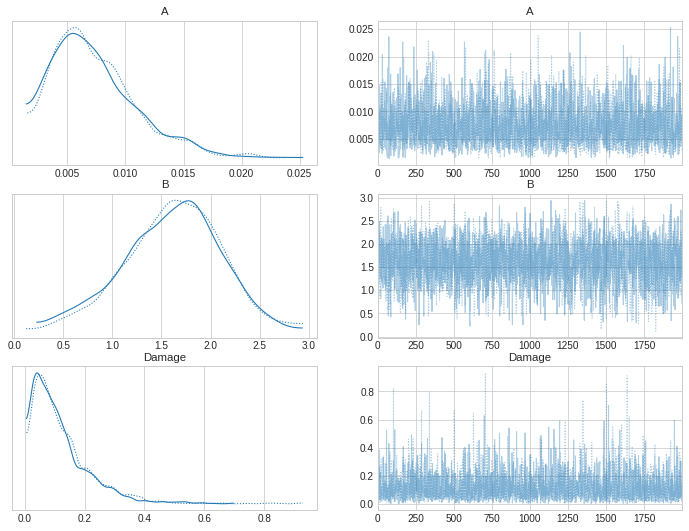
\includegraphics[width=\linewidth]{Figures/bayesianInferenceV3.png}
	\caption{Posterior distributions of parameters $A$, $B$ after 5 iterations of Bayesian Inference and \gls{NUTS}}
	\label{bayesInfno5}
\end{figure}

A typical example of \gls{NUTS} is depicted in Figure \ref{bayesInfno5}, using two Markov chains and 4000 samples. What is more, the updating of the parameters' distribution through 20 iterations is illustrated in Figure \ref{posteriorsAfter20Iterations}, highlighting the effect of including observations in order to define more accurately the stochastic parameters of the deterioration model. 

\begin{figure}[H]
    \centering
    \begin{subfigure}[b]{0.48\textwidth}
        \centering
        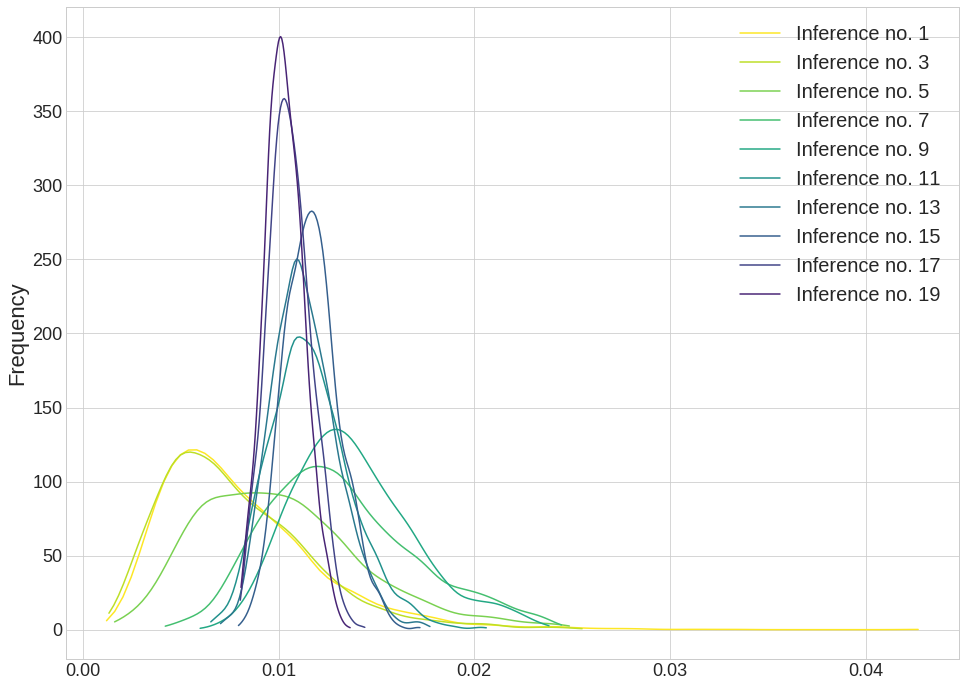
\includegraphics[width=\textwidth]{Figures/inferenceA.png}
        \caption{Posterior distribution of $A$}
        \label{postA20iters}
    \end{subfigure}
    \hfill
    \begin{subfigure}[b]{0.48\textwidth}
        \centering
        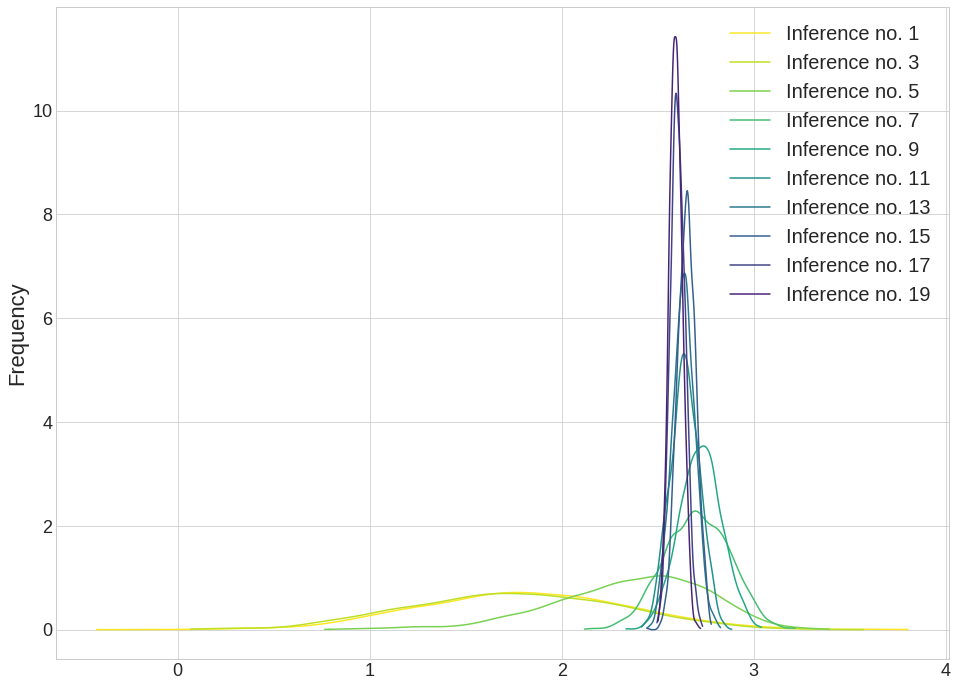
\includegraphics[width=\textwidth]{Figures/inferenceB.png}
        \caption{Posterior distribution of $B$}
        \label{postB20iters}
    \end{subfigure}
    \caption{Posterior distributions of parameters $A$, $B$ during 20 iteration of Bayesian Inference and \gls{NUTS}}
    \label{posteriorsAfter20Iterations}
\end{figure}

\newpage

%------------------------------------------------------------------------------
%	DRL ALGORITHM VALIDATION
%------------------------------------------------------------------------------

\subsubsection{\acrfull{DRL} algorithms}

Before proceeding to more complicated cases, the three \gls{DRL} algorithms, namely \gls{DDQN}, \gls{A2C} and \gls{PPO}, will be tested and compared on the CartPole-v0\footnotemark environment. The results, i.e. the rewards that the agent received over the episodes, during its training, are displayed in Figure \ref{allAlgsCart}.\\

\footnotetext{More information on the CartPole-v0 environment can be found \href{http://gym.openai.com/envs/CartPole-v0/}{here}.}

\begin{figure}[H]
    \centering
    \begin{subfigure}[b]{0.48\textwidth}
        \centering
        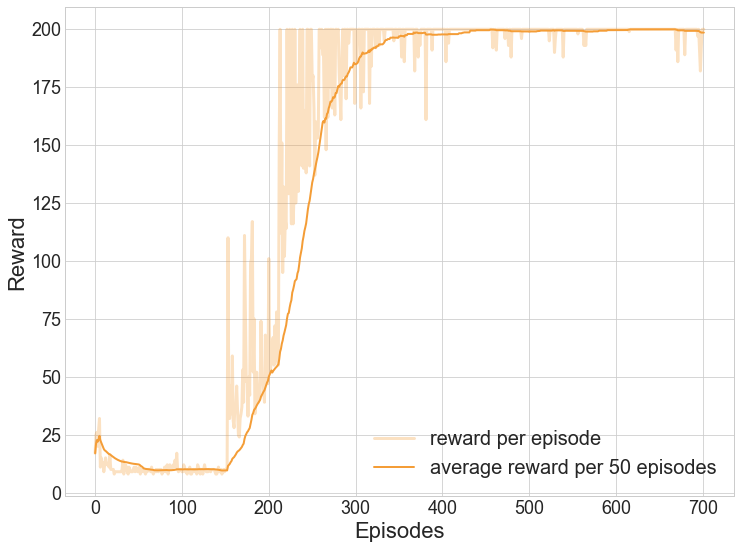
\includegraphics[width=\textwidth]{Figures/ddqnCart.png}
        \caption{\gls{DDQN}}
        \label{ddqnCart}
    \end{subfigure}
    \begin{subfigure}[b]{0.48\textwidth}
        \centering
        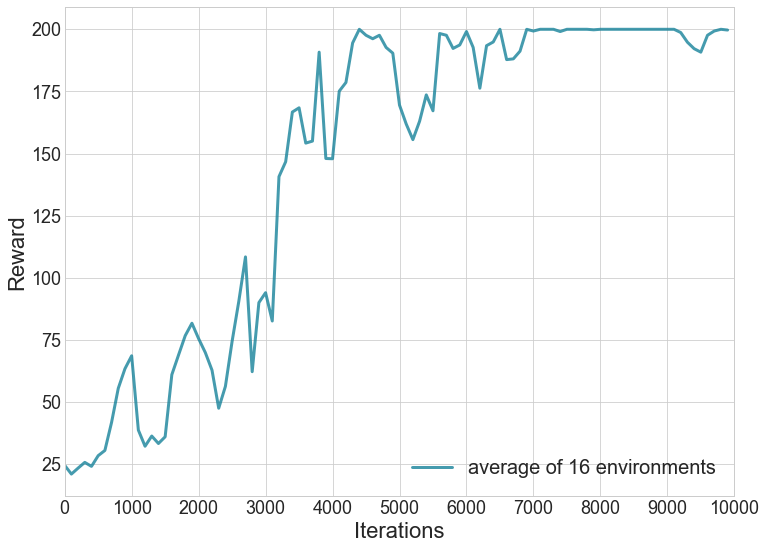
\includegraphics[width=\textwidth]{Figures/a2cCart.png}
        \caption{\gls{A2C}}
        \label{a2cCart}
    \end{subfigure}
    \hfill
    \begin{subfigure}[b]{0.48\textwidth}
        \centering
        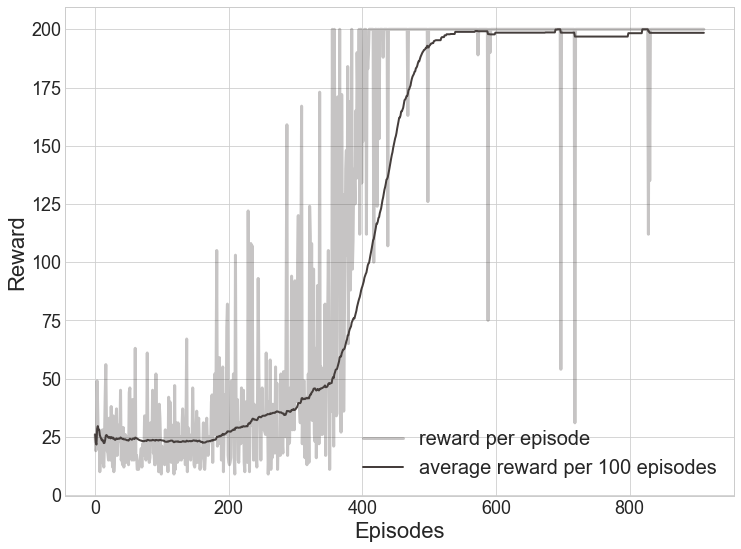
\includegraphics[width=\textwidth]{Figures/ppoCart.png}
        \caption{\gls{PPO}}
        \label{ppoCart}
    \end{subfigure}
    \caption{All three algorithms on the CartPole-v0 environment}
    \label{allAlgsCart}
\end{figure}

It should be noted that the \acrfull{A2C} algorithm performed sufficiently in the CartPole-v0 environment this is why it is included in Figure \ref{allAlgsCart}. Unfortunately, this was not the case for the toy problem. Its stability is also ambiguous, since out of the three algorithms it was the slower one to reach the optimal CartPole-v0 reward.

\newpage

%------------------------------------------------------------------------------
%	BENCHMARKING
%------------------------------------------------------------------------------

\subsection{Benchmarking} \label{toyBenchSec}

Even if the algorithms converge to theoretically optimal values for the examined cases, the superiority of the proposed framework will be highlighted upon comparison with a benchmark value. Defining such a value is cumbersome and computationally expensive due to the stochastic nature of the problem (both discrete and continuous). \\

More often than not, a heuristic threshold based approach is being used, accounting for various control quantities, such as the maximum acceptable damage, the most beneficial periodic maintenance time interval or the maximum probability of failure allowed \cite{keizer2017condition}, \cite{grall2002condition}, \cite{barone2014reliability}, \cite{li2015time}. For the current application, both in the discrete and in the continuous case, a fine grid of repair and replace damage values were tested, in order to determine when would be the most beneficial to intervene in the deterioration of the \gls{SDOF} oscillator. For each combination of values, a plethora of episodes was ran, due to the high stochasticity. In the discrete case the variance was not significant, thus, only the expected value of the cost is included in the results. The obtained thresholds and costs are displayed in Table \ref{benchValues}.

\begin{table}[H]
    \centering
    \caption{Benchmark maintenance thresholds and costs - Toy Problem}
    \label{benchValues}
    \begin{tabular}{lccccc}
                            & \multicolumn{2}{c}{\textbf{Optimal Thresholds}} &                    &                                       \\ \toprule
                            & \textbf{Repair}        & \textbf{Replace}       & \textbf{Mean Cost} & \multicolumn{1}{c}{\textbf{St. Dev.}} & \textbf{Failure Damage} \\ \midrule
        \textbf{Discrete}   & None                   & $0.14$                   & $\boldsymbol{21809.37}$  & - & $0.5$ \\
        \textbf{Continuous} & $0.05$ & $0.10$ & $\boldsymbol{80745.31}$  & $22658.95$ & $0.2$ \\ \bottomrule                         
    \end{tabular}
\end{table}

To further elaborate on the findings presented in Table \ref{benchValues}, for the discrete case there was no scenario where it was beneficial to perform a repair, thus, only the replace value is relevant. It is worth mentioning that due to the parameter updating in a closed form that is possible in the discrete case, more decision steps were accounted for, thus, a higher damage failure value was considered.

%------------------------------------------------------------------------------
%	RESULTS
%------------------------------------------------------------------------------

\newpage

\subsection{Results} \label{resultsToySec}

%------------------------------------------------------------------------------
%	DISCRETE RESULTS
%------------------------------------------------------------------------------

Prior to presenting the results for the toy problem, in order for them to be reproducible, the hyper-parameters used for both the discrete and continuous variations are displayed in Tables \ref{ddqnHyperToy} and \ref{ppoHyperToy}, for \gls{DDQN} and \gls{PPO} respectively.

\begin{table}[H]
    \centering
    \caption{\gls{DDQN} hyperparameters - Toy problem}
    \label{ddqnHyperToy}
    \begin{tabular}{lcc}
        \toprule
        \textbf{Hyper-parameter} & \multicolumn{1}{l}{\textbf{Discrete}} & \multicolumn{1}{l}{\textbf{Continuous}} \\ \midrule
        gamma, $\gamma$ & $0.99$ & $0.99$ \\
        learning rate & $5.00\mathrm{E}-3$ & $1.00\mathrm{E}-2$ \\
        number of inner layers & $2$ & $2$ \\
        size of inner layers & $128$ & $128$ \\
        start epsilon, $\epsilon$  & $1.0$ & $1.0$ \\
        batch size & $64$ & $128$ \\ \bottomrule
    \end{tabular}
\end{table}

\begin{table}[H]
    \centering
    \caption{\gls{PPO} hyper-parameters - Toy problem}
    \label{ppoHyperToy}
    \begin{tabular}{lcc}
        \toprule
        \textbf{Hyper-parameter} & \multicolumn{1}{l}{\textbf{Discrete}} & \multicolumn{1}{l}{\textbf{Continuous}} \\ \midrule
        gamma, $\gamma$ & $0.99$ & $0.99$ \\
        clip ratio & $0.2$ & $0.1$ \\
        lambda, $\lambda$ & $0.95$ & $0.95$ \\
        number of inner layers & $2$ & $2$ \\
        size of inner layers & $256$ & $256$ \\
        policy learning rate & $1.00\mathrm{E}-4$ & $1.00\mathrm{E}-3$ \\
        value function learning rate & $5.00\mathrm{E}-4$ & $5.00\mathrm{E}-3$ \\ \bottomrule
    \end{tabular}
\end{table}


It should be noted that the number and the dimensions of the inner hidden layers were the same both for the actor and the critic network in the case of \gls{PPO}. What is more, regarding the neural network activation function, for all networks of this project, and all layers, the \gls{ReLU} function is chosen.

\subsubsection{Discrete case}

Combining the aforementioned aspects regarding the proposed framework and the toy problem, the \gls{DRL} algorithms \gls{DDQN} and \gls{PPO} managed to yield optimal strategies that even outperform the benchmark solution. In Figure \ref{discreteAllAlgs}, the training of the agent is illustrated, by plotting the cost of the maintenance for a life cycle of 50 decision steps over the episodes ran during training.

\begin{figure}[H] 
    \centering
	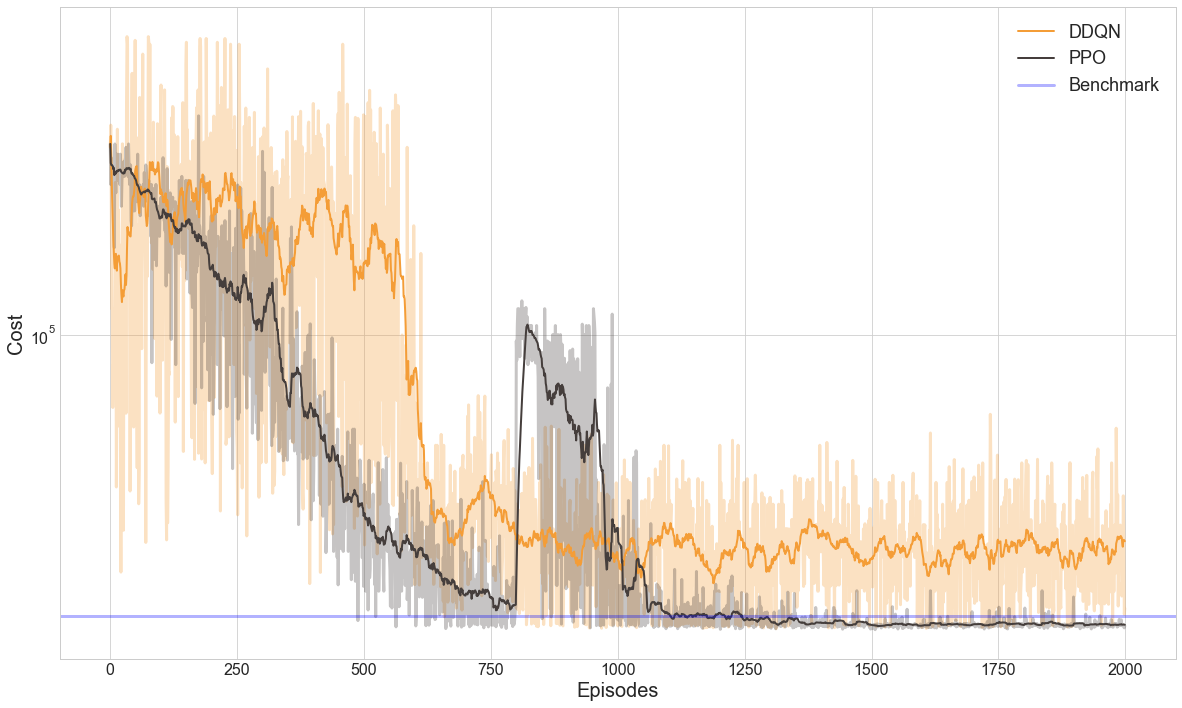
\includegraphics[width=\linewidth]{Figures/discreteAllAlgs.png}
	\caption{\gls{DDQN} and \gls{PPO} on discrete \gls{SDOF} environment}
	\label{discreteAllAlgs}
\end{figure}


It should be noted, that owing to the low complexity of this introductory application, it was probable that the \gls{DRL} approach would not necessarily achieve a lower maintenance cost. However, it can be observed in Figure \ref{discreteAllAlgs}, that \gls{PPO} performs slightly better. The superiority of \gls{PPO} can be also complimented by its significantly lower variance, even though the environment is still stochastic. Another interesting finding for interpretation are the policies that were found by the agent. These policy realizations are plotted in Figure \ref{discretePolicy}.

\begin{figure}[H]
    \centering
	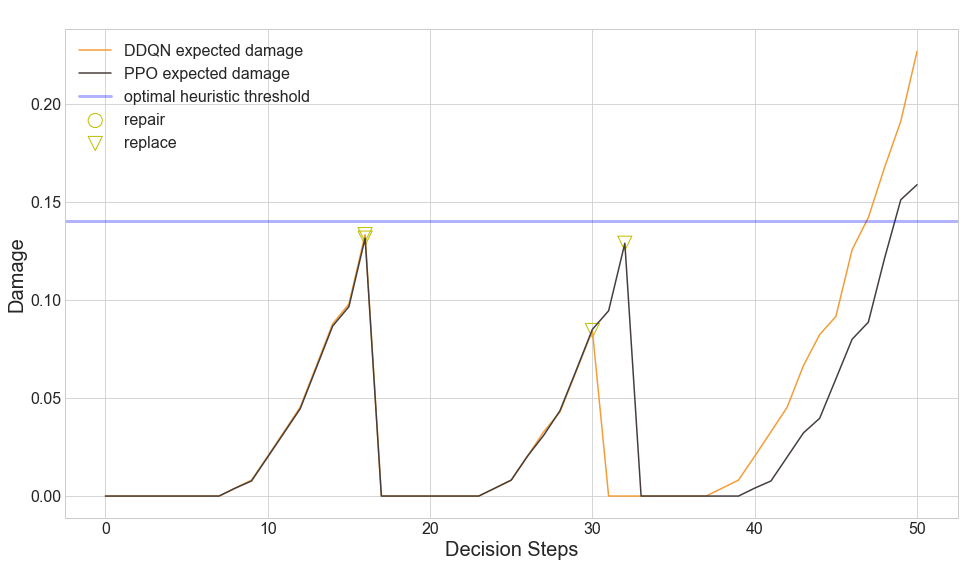
\includegraphics[width=\linewidth]{Figures/discretePolicies.png}
	\caption{\gls{DDQN} and \gls{PPO} policy realizations on discrete \gls{SDOF} environment}
	\label{discretePolicy}
\end{figure}

As it can be seen in the above plot, both the \gls{DDQN} and \gls{PPO} agents, managed to find a more suitable damage threshold to perform the replace action. The fact that \gls{DDQN} fails to consistently choose when it is more beneficial to replace the component, as seen at decision step 30, leads to the slightly worse performance of the agent. On the other hand, \gls{PPO} seems to be more stable and able to achieve lower maintenance costs, by performing a replace action when the damages reaches a value around 0.13.\\

Lastly, both the tested algorithms, avoid to perform a partial repair action, which is a fact backed up also by the benchmark runs. In this discrete setup of the toy problem, repairing the \gls{SDOF} oscillator unarguably leads to higher maintenance costs.

%------------------------------------------------------------------------------
%	CONTINUOUS RESULTS
%------------------------------------------------------------------------------

\subsubsection{Continuous case}

Proceeding to the more accurate, from a modelling standpoint, continuous version of the toy problem, it is more evident that the proposed framework leads to optimal maintenance strategies in such stochastic environments. Prior to showcasing the performance of the tested algorithms, it should be mentioned that due to computational costs and time-consuming runs, the decision steps were reduced to 20 (instead of 50 for the discrete case), and the failure damage threshold was now assumed to be 0.2 (instead of 0.5 for the discrete case) as shown also in Table \ref{toyInput}. The reduction in the damage threshold was made in order for the \gls{SDOF} oscillator to deteriorate enough so as the cost linked to the probability of failure to be substantial. The training of the agent is plotted over the episodes in Figure \ref{continuousAllAlgs}.

\begin{figure}[H]
    \centering
	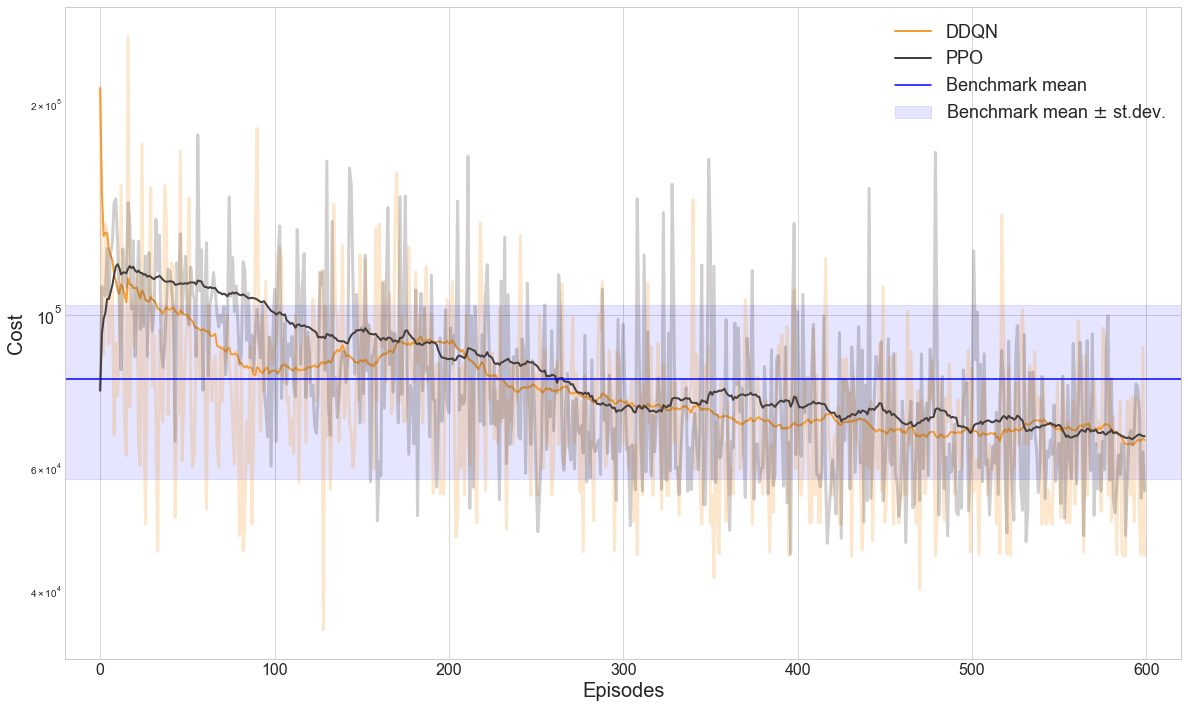
\includegraphics[width=\linewidth]{Figures/continuousAllAlgs.png}
	\caption{\gls{DDQN} and \gls{PPO} on continuous \gls{SDOF} environment}
	\label{continuousAllAlgs}
\end{figure}

It is evident that both the \gls{DDQN} and the \gls{PPO} algorithms outperform the benchmark approach. The exact details of this comparison are included in Table \ref{costsContinuous}. Apart from the mean value and the standard deviation regarding the cost of each approach, the last column of the table contains the reduction in cost (as a percentage) compared with the traditional heuristic solution (benchmark). Additionally, one can observe that in the case of the benchmark, the variability in costs is significantly higher. This means that the stochasticity of the environment can lead to poor performance and higher costs, when following a threshold based policy, which is not the case when applying the proposed framework.

\begin{table}[H]
    \centering
    \caption{\gls{DRL} algorithms' performance on continuous Toy Problem}
    \label{costsContinuous}
    \begin{tabular}{lccc}
        & \multicolumn{2}{c}{\textbf{Last 50   Episodes}} & \\ \toprule
        \textbf{\gls{DRL} Algorithm} & \textbf{Mean Cost} & \textbf{St. Dev. Cost} & \textbf{Cost Decrease} \\ \toprule
        Benchmark & 80745.3 & 22659.0 & - \\
        \gls{DDQN} & 63776.0 & 14773.7 & 21.02\% \\
        \gls{PPO} & 64602.0 & 12992.6 & 19.99\% \\ \bottomrule
    \end{tabular}
\end{table}

Owing to the extensively mentioned stochasticity of the environment, it is expected that each episode which was ran, will differ considerably from one another. Therefore, a single policy realization would not be a representative illustration, to fully understand the training of the agent. Nevertheless, for the shake of comparison between the two algorithms and the benchmark thresholds, such realizations over the 20 decision steps are plotted in Figure \ref{continuousPolicy}.

\begin{figure}[H]
    \centering
	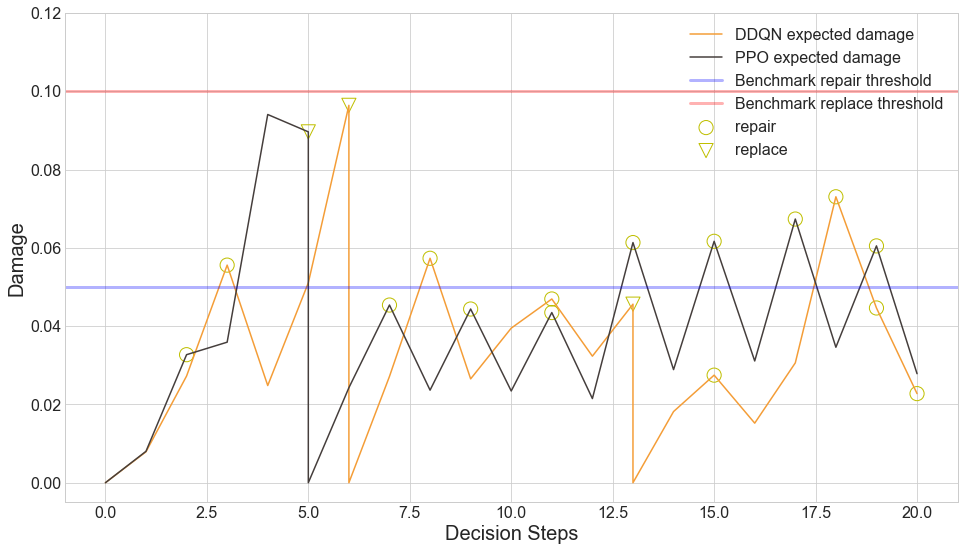
\includegraphics[width=\linewidth]{Figures/continuousPolicies.png}
	\caption{\gls{DDQN} and \gls{PPO} policy realizations on continuous \gls{SDOF} environment}
	\label{continuousPolicy}
\end{figure}

It is observed for both algorithms that the expected damage does not overcome the replace benchmark threshold of $0.10$. Additionally the damage value when the agent chooses to perform a partial repair fluctuates around the heuristic benchmark value. More specifically, regarding \gls{PPO}, when the damage increases in a more steep and unexpected way such as in decision step 4, the agent chooses to permit that and not proceed with a repair, letting the system deteriorate up to higher values and then performs a complete replacement. This is not strictly the case for \gls{DDQN}, as it can be seen that for lower damage values like the one during decision step 13, the agent chose to perform a replacement action even though the damage was smaller than the repair benchmark threshold of $0.05$. This constitutes an interesting finding, since both agents achieved almost identical costs, which is something that can be possible attributed to the high stochasticity of the corrosive environment. 

\newpage

More descriptive conclusion could be possibly drawn if more than one episodes, hence policies, were to be plotted. This is done for both \gls{DDQN} and \gls{PPO} in Figures \ref{polDDQN} and \ref{polPPO} respectively.

\begin{figure}[H]
    \centering
	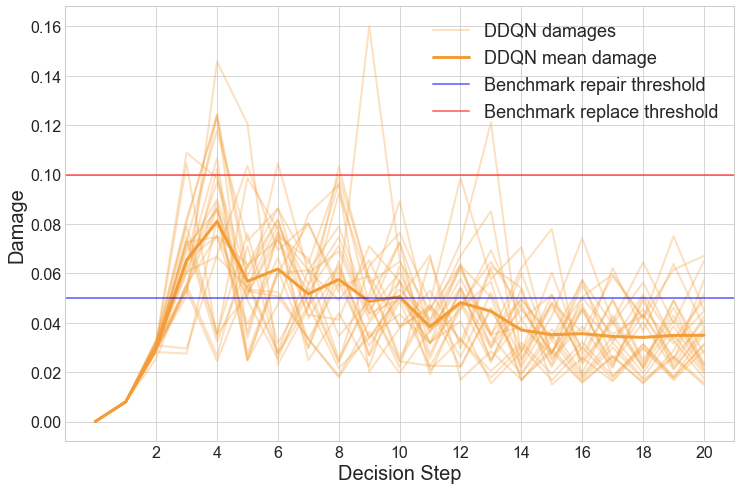
\includegraphics[width=0.75\linewidth]{Figures/policiesDDQNmean.png}
	\caption{Probability of failure for 50 policy realizations, for both \gls{DDQN} and \gls{PPO}}
	\label{polDDQN}
\end{figure}

\begin{figure}[H]
    \centering
	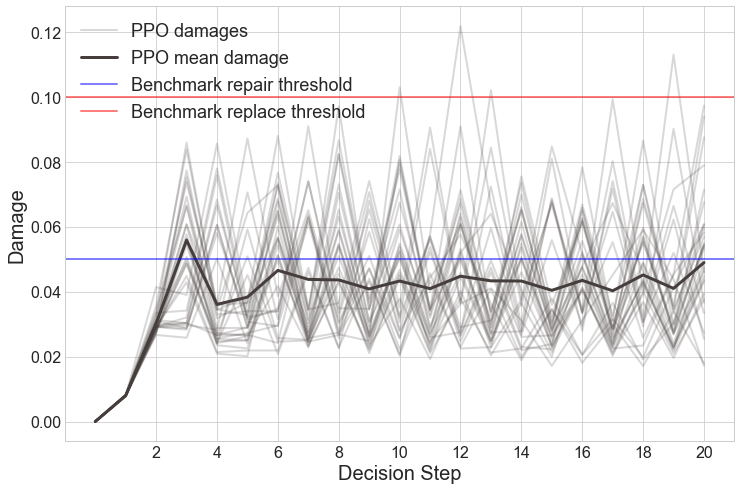
\includegraphics[width=0.75\linewidth]{Figures/policiesPPOmean.png}
	\caption{Probability of failure for 50 policy realizations, for both \gls{DDQN} and \gls{PPO}}
	\label{polPPO}
\end{figure}

In these plots, policy trends can be identified, highlighting once more the ability of the agent to diverge from the traditional heuristic actions and proceed in taking actions at unexpected stages of the deterioration. It should be mentioned that the plotted policies, even though they do not lead to the minimum of maintenance costs, they are all still smaller than the benchmark average one. Elaborating further on the degree to which the obtained policies comply with the benchmark values, it can be stated that \gls{PPO} chose actions in a considerably more consistent way compared to \gls{DDQN}, with only limited policies passing the replace heuristic value, and the vast majority of the repair actions being performed for damages lower than the repair threshold. This is concluded from the steep peaks that have formed inside the band between $0.05$ and $0.10$, namely the repair and replace benchmark values. Even though these peaks could indicate a periodic pattern of maintenance, particularly replace ones, this is not the case, since they belong to different episodes. On the contrary, even though the \gls{DDQN} agent restrict the damage mostly below the replace threshold, it is observed that the obtained policies are more stochastic, with many repair actions taking place even at times where the damages approaches $0.10$, i.e. the replace heuristic value. An important issue, that is probably responsible for these differences among the two algorithms, is the way the agent chooses actions in each case. In \gls{DDQN} the agent picks deterministically the action it considers the most beneficial, based solely on the action-state value functions $Q(a_t, s_t)$. On the other hand, the \gls{PPO} agent, even if the damages has reached a worrying damage value, chooses the action based on a probability distribution, i.e. the policy $\pi(a_t \mid s_t)$ which makes every action, no matter how "good" or "bad" is, to still stand some chances of being picked.\\

Another interesting outcome of the proposed framework is the impact of the updating procedure, in case the "true" values of the parameters $A, B$ are known. In Figures \ref{aUpdate}, \ref{bUpdate}, the evolution of $A$ and $B$ respectively, is plotted along the decision steps, for 9 different episodes.

\begin{figure}[H]
    \centering
	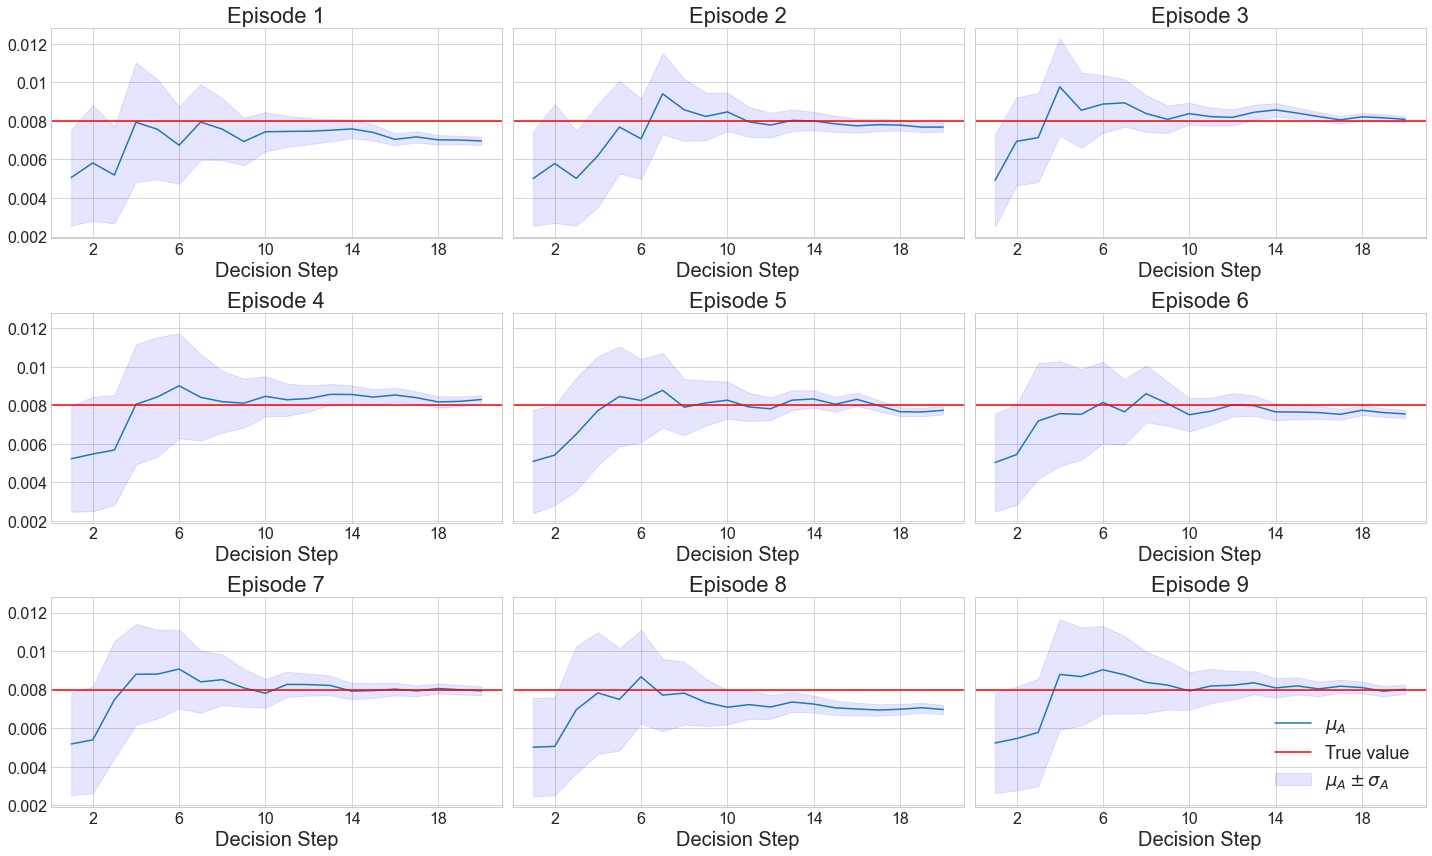
\includegraphics[width=\linewidth]{Figures/aInference.png}
	\caption{Updating of parameter $A$ for nine (9) of the episodes}
	\label{aUpdate}
\end{figure}

\begin{figure}[H]
    \centering
	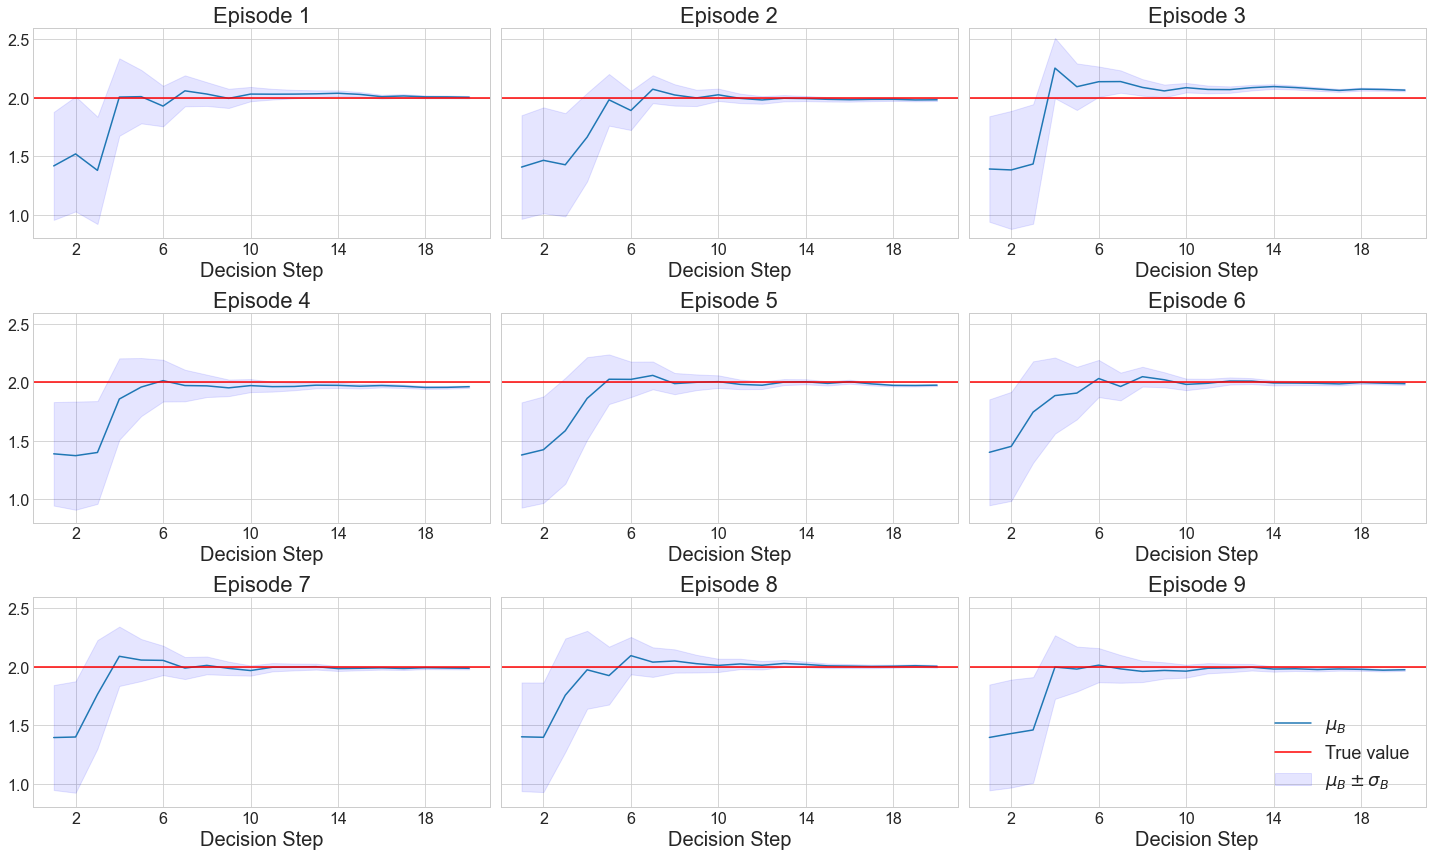
\includegraphics[width=\linewidth]{Figures/bInference2.png}
	\caption{Updating of parameter $B$ for nine (9) of the episodes}
	\label{bUpdate}
\end{figure}

It can be safely concluded that incorporating more noisy observations, which have been generated using the assumed ``true'' values for $A$ and $B$, i.e. $0.008$ and $2.0$, reduces the uncertainty, and the stochastic parameters indeed converge over time with an ever decreasing variance. It should be noted though that for limited cases the inferred value of the parameters seem to converge to a slightly offset value, such as in episodes 1, 8 in Figure \ref{aUpdate}, and in episode 3 in Figure \ref{bUpdate}. This anomaly could be justified by the limited amount of decision steps that was employed, expecting a better convergence to the expected ``true'' values if more updates were performed.

\newpage

Lastly, since the cost linked to the risk of failure, and subsequently the probability of failure, have an important contribution to the total reward/cost of an episode, this probability is being plotted over the 20 decision steps for a plethora of episodes (50 in total) in Figure \ref{pfs}.

\begin{figure}[H]
    \centering
    \begin{subfigure}[b]{0.48\textwidth}
        \centering
        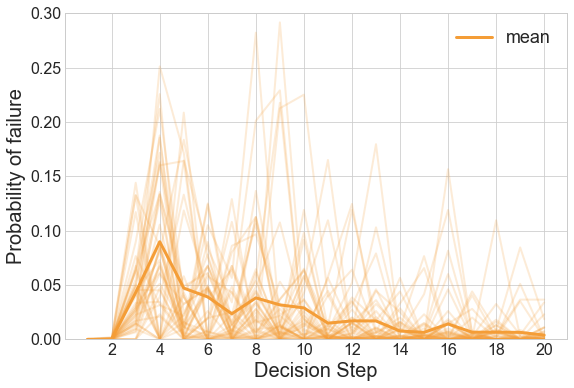
\includegraphics[width=\textwidth]{Figures/pfsDDQN.png}
        \caption{\gls{DDQN}}
        \label{pfDDQN}
    \end{subfigure}
    \begin{subfigure}[b]{0.48\textwidth}
        \centering
        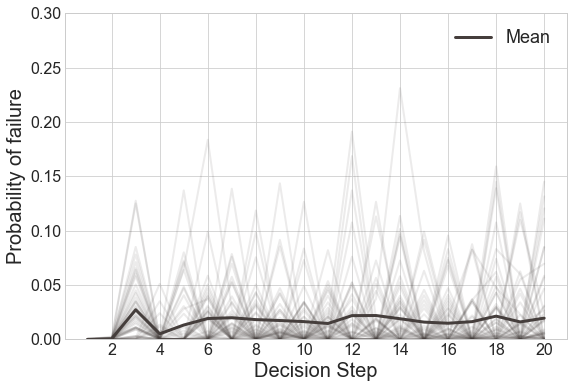
\includegraphics[width=\textwidth]{Figures/pfsPPO.png}
        \caption{\gls{PPO}}
        \label{pfPPO}
    \end{subfigure}
    \caption{Probability of failure for 50 policy realizations}
    \label{pfs}
\end{figure}

Similar conclusions that have already been drawn for the comparison between \gls{DDQN} and \gls{PPO} can be supported through the probability of failure plots, too. \gls{PPO} appears to perform in a more controlled manner, not allowing the probability of failure, $P_f$, hence, the cost $C_{\text{risk}}$ to grow excessively. Observing also the mean of these episodes, it can be deduced that the agent forces the risk of failure to stay approximately constant, especially for later steps (after the fifth one), and in total it does not allow $P_f$ to overcome the value of $0.035$. This is not the case for \gls{DDQN}, as seen in Figure \ref{pfDDQN}, where especially for the early steps, the agent is not that strict, allowing even higher values for the cost associated with the risk of failure. Among the two algorithms, the maintenance strategies according to \gls{DDQN} could be considered more reasonable, since taking early maintenance decision is counter-intuitive for a brand new engineering system. However, controlling the damage from an early stage, seems to work as well, leading to relatively stable results, as \gls{PPO} showcases.

%------------------------------------------------------------------------------
%	CONCLUSIONS
%------------------------------------------------------------------------------

\subsection{Conclusions}

Concluding this chapter, a review of the obtained results for the toy problem will be made, while some summarizing comments and conclusions will be drawn. \\

Starting from the discrete case, due to the great simplifications in the modelling of the system's deterioration and the state and observation spaces, it was feasible to derive optimal maintenance strategies even with a heuristic damage threshold-based approach. Nonetheless, \gls{PPO} managed to outperform the benchmark approach and arrived to a slightly better policy, showcasing the superiority of the proposed framework even for such trivial cases.\\

Moving to the more realistic continuous version of the toy problem, it can be safely concluded that the developed tool performed significantly better. Both \gls{DDQN} and \gls{PPO} managed to yield an optimal sequence of maintenance actions, which decreased the total cost over the system's lifetime b approximately $20\%$ (the exact numbers/costs and the training of the agents can be found at Table \ref{costsContinuous} and Figure \ref{continuousAllAlgs} respectively).\\


Unfortunately, the \gls{A2C} algorithm was not able to perform adequately, this is why it is disregarded from the rest of the thesis. A possible reason for its poor performance can be its instability, especially in such a stochastic environment. After all, this is the main reason algorithms like \gls{TRPO} and especially \gls{PPO} were developed; to provide a more stable learning while still taking advantage of the benefits of a policy gradient algorithm \cite{schulman2017proximal}.
